\documentclass{beamer}

\mode<presentation> {
\usetheme{CambridgeUS}
\usecolortheme{lily}
}

\usepackage{graphicx}
\graphicspath{{../}, {./}}
\usepackage{color}

\usepackage[T1]{fontenc}
\usepackage[sc,osf]{mathpazo}

% Linux Libertine FontType for main text
\usepackage{fontspec,xltxtra,xunicode}
\setromanfont[Mapping=tex-text]{Linux Libertine} % Main document font

% use ding font
\usepackage{pifont}

% subfigure and adjustbox
\usepackage{caption}
\usepackage{subcaption}
\usepackage{adjustbox}


\usepackage{array}
% New column type with fixed width,
% centering both horizontally and vertically
\newcolumntype{M}[1]{>{\centering\arraybackslash\hspace{0pt}}m{#1}}

% tikz
\usepackage{tikz}
\usetikzlibrary{arrows, positioning, shapes, decorations.pathmorphing}
% This is not an official TikZ library. Use at your own risk!

\makeatletter
% alternative latex arrow
\pgfarrowsdeclare{latexnew}{latexnew}
{
  \ifdim\pgfgetarrowoptions{latexnew}=-1pt%
    \pgfutil@tempdima=0.28pt%
    \pgfutil@tempdimb=\pgflinewidth%
    \ifdim\pgfinnerlinewidth>0pt%
      \pgfmathsetlength\pgfutil@tempdimb{.6\pgflinewidth-.4*\pgfinnerlinewidth}%
    \fi%
    \advance\pgfutil@tempdima by.3\pgfutil@tempdimb%
  \else%
    \pgfutil@tempdima=\pgfgetarrowoptions{latexnew}%
    \divide\pgfutil@tempdima by 10%
  \fi%
  \pgfarrowsleftextend{+-1\pgfutil@tempdima}%
  \pgfarrowsrightextend{+9\pgfutil@tempdima}%
}
{
  \ifdim\pgfgetarrowoptions{latexnew}=-1pt%
    \pgfutil@tempdima=0.28pt%
    \pgfutil@tempdimb=\pgflinewidth%
    \ifdim\pgfinnerlinewidth>0pt%
      \pgfmathsetlength\pgfutil@tempdimb{.6\pgflinewidth-.4*\pgfinnerlinewidth}%
    \fi%
    \advance\pgfutil@tempdima by.3\pgfutil@tempdimb%
  \else%
    \pgfutil@tempdima=\pgfgetarrowoptions{latexnew}%
    \divide\pgfutil@tempdima by 10%
    \pgfsetlinewidth{0bp}%
  \fi%
  \pgfpathmoveto{\pgfqpoint{9\pgfutil@tempdima}{0pt}}
  \pgfpathcurveto
  {\pgfqpoint{6.3333\pgfutil@tempdima}{.5\pgfutil@tempdima}}
  {\pgfqpoint{2\pgfutil@tempdima}{2\pgfutil@tempdima}}
  {\pgfqpoint{-1\pgfutil@tempdima}{3.75\pgfutil@tempdima}}
  \pgfpathlineto{\pgfqpoint{-1\pgfutil@tempdima}{-3.75\pgfutil@tempdima}}
  \pgfpathcurveto
  {\pgfqpoint{2\pgfutil@tempdima}{-2\pgfutil@tempdima}}
  {\pgfqpoint{6.3333\pgfutil@tempdima}{-.5\pgfutil@tempdima}}
  {\pgfqpoint{9\pgfutil@tempdima}{0pt}}
  \pgfusepathqfill
}

% alternative latex reversed arrow
\pgfarrowsdeclarereversed{latexnew reversed}{latexnew reversed}{latexnew}{latexnew}

% alternative latex' arrow
\pgfarrowsdeclare{latex'new}{latex'new}
{
  \ifdim\pgfgetarrowoptions{latex'new}=-1pt%
    \pgfutil@tempdima=0.28pt%
    \advance\pgfutil@tempdima by.3\pgflinewidth%
  \else%
    \pgfutil@tempdima=\pgfgetarrowoptions{latex'new}%
    \divide\pgfutil@tempdima by 10%
  \fi%
  \pgfarrowsleftextend{+-4\pgfutil@tempdima}
  \pgfarrowsrightextend{+6\pgfutil@tempdima}
}
{
  \ifdim\pgfgetarrowoptions{latex'new}=-1pt%
    \pgfutil@tempdima=0.28pt%
    \advance\pgfutil@tempdima by.3\pgflinewidth%
  \else%
    \pgfutil@tempdima=\pgfgetarrowoptions{latex'new}%
    \divide\pgfutil@tempdima by 10%
    \pgfsetlinewidth{0bp}%
  \fi%
  \pgfpathmoveto{\pgfqpoint{6\pgfutil@tempdima}{0\pgfutil@tempdima}}
  \pgfpathcurveto
  {\pgfqpoint{3.5\pgfutil@tempdima}{.5\pgfutil@tempdima}}
  {\pgfqpoint{-1\pgfutil@tempdima}{1.5\pgfutil@tempdima}}
  {\pgfqpoint{-4\pgfutil@tempdima}{3.75\pgfutil@tempdima}}
  \pgfpathcurveto
  {\pgfqpoint{-1.5\pgfutil@tempdima}{1\pgfutil@tempdima}}
  {\pgfqpoint{-1.5\pgfutil@tempdima}{-1\pgfutil@tempdima}}
  {\pgfqpoint{-4\pgfutil@tempdima}{-3.75\pgfutil@tempdima}}
  \pgfpathcurveto
  {\pgfqpoint{-1\pgfutil@tempdima}{-1.5\pgfutil@tempdima}}
  {\pgfqpoint{3.5\pgfutil@tempdima}{-.5\pgfutil@tempdima}}
  {\pgfqpoint{6\pgfutil@tempdima}{0\pgfutil@tempdima}}
  \pgfusepathqfill
}

% alternative latex' reversed arrow
\pgfarrowsdeclarereversed{latex'new reversed}{latex'new reversed}{latex'new}{latex'new}

% alternative o arrow
\pgfarrowsdeclare{onew}{onew}
{
  \pgfarrowsleftextend{+-.5\pgflinewidth}
  \ifdim\pgfgetarrowoptions{onew}=-1pt%
    \pgfutil@tempdima=0.4pt%
    \advance\pgfutil@tempdima by.2\pgflinewidth%
    \pgfutil@tempdimb=9\pgfutil@tempdima\advance\pgfutil@tempdimb by.5\pgflinewidth%
    \pgfarrowsrightextend{+\pgfutil@tempdimb}%
  \else%
    \pgfutil@tempdima=\pgfgetarrowoptions{onew}%
    \advance\pgfutil@tempdima by -0.5\pgflinewidth%
    \pgfarrowsrightextend{+\pgfutil@tempdima}%
  \fi%
}
{ 
  \ifdim\pgfgetarrowoptions{onew}=-1pt%
    \pgfutil@tempdima=0.4pt%
    \advance\pgfutil@tempdima by.2\pgflinewidth%
    \pgfutil@tempdimb=0pt%
  \else%
    \pgfutil@tempdima=\pgfgetarrowoptions{onew}%
    \divide\pgfutil@tempdima by 9%
    \pgfutil@tempdimb=0.5\pgflinewidth%
  \fi%
  \pgfsetdash{}{+0pt}
  \pgfpathcircle{\pgfpointadd{\pgfqpoint{4.5\pgfutil@tempdima}{0bp}}%
                             {\pgfqpoint{-\pgfutil@tempdimb}{0bp}}}%
                {4.5\pgfutil@tempdima-\pgfutil@tempdimb}%
  \pgfusepathqstroke
}

% alternative square arrow
\pgfarrowsdeclare{squarenew}{squarenew}
{
 \ifdim\pgfgetarrowoptions{squarenew}=-1pt%
   \pgfutil@tempdima=0.4pt
   \advance\pgfutil@tempdima by.275\pgflinewidth%
   \pgfarrowsleftextend{+-\pgfutil@tempdima}
   \advance\pgfutil@tempdima by.5\pgflinewidth
   \pgfarrowsrightextend{+\pgfutil@tempdima}
 \else%
   \pgfutil@tempdima=\pgfgetarrowoptions{squarenew}%
   \divide\pgfutil@tempdima by 8%
   \pgfarrowsleftextend{+-7\pgfutil@tempdima}%
   \pgfarrowsrightextend{+1\pgfutil@tempdima}%
 \fi%
}
{
 \ifdim\pgfgetarrowoptions{squarenew}=-1pt%
   \pgfutil@tempdima=0.4pt%
   \advance\pgfutil@tempdima by.275\pgflinewidth%
   \pgfutil@tempdimb=0pt%
 \else%
   \pgfutil@tempdima=\pgfgetarrowoptions{squarenew}%   
   \divide\pgfutil@tempdima by 8%
   \pgfutil@tempdimb=0.5\pgflinewidth%
 \fi%
 \pgfsetdash{}{+0pt}
 \pgfsetroundjoin
 \pgfpathmoveto{\pgfpointadd{\pgfqpoint{1\pgfutil@tempdima}{4\pgfutil@tempdima}}
                            {\pgfqpoint{-\pgfutil@tempdimb}{-\pgfutil@tempdimb}}}
 \pgfpathlineto{\pgfpointadd{\pgfqpoint{-7\pgfutil@tempdima}{4\pgfutil@tempdima}}
                            {\pgfqpoint{\pgfutil@tempdimb}{-\pgfutil@tempdimb}}}
 \pgfpathlineto{\pgfpointadd{\pgfqpoint{-7\pgfutil@tempdima}{-4\pgfutil@tempdima}}
                            {\pgfqpoint{\pgfutil@tempdimb}{\pgfutil@tempdimb}}}
 \pgfpathlineto{\pgfpointadd{\pgfqpoint{1\pgfutil@tempdima}{-4\pgfutil@tempdima}}
                            {\pgfqpoint{-\pgfutil@tempdimb}{\pgfutil@tempdimb}}}
 \pgfpathclose
 \pgfusepathqfillstroke
}

% alternative stealth arrow
\pgfarrowsdeclare{stealthnew}{stealthnew}
{
  \ifdim\pgfgetarrowoptions{stealthnew}=-1pt%
    \pgfutil@tempdima=0.28pt%
    \pgfutil@tempdimb=\pgflinewidth%
    \ifdim\pgfinnerlinewidth>0pt%
      \pgfmathsetlength\pgfutil@tempdimb{.6\pgflinewidth-.4*\pgfinnerlinewidth}%
    \fi%
    \advance\pgfutil@tempdima by.3\pgfutil@tempdimb%
  \else%
    \pgfutil@tempdima=\pgfgetarrowoptions{stealthnew}%
    \divide\pgfutil@tempdima by 8%
  \fi%
  \pgfarrowsleftextend{+-3\pgfutil@tempdima}
  \pgfarrowsrightextend{+5\pgfutil@tempdima}
}
{
  \ifdim\pgfgetarrowoptions{stealthnew}=-1pt%
    \pgfutil@tempdima=0.28pt%
    \pgfutil@tempdimb=\pgflinewidth%
    \ifdim\pgfinnerlinewidth>0pt%
      \pgfmathsetlength\pgfutil@tempdimb{.6\pgflinewidth-.4*\pgfinnerlinewidth}%
    \fi%
    \advance\pgfutil@tempdima by.3\pgfutil@tempdimb%
  \else%
    \pgfutil@tempdima=\pgfgetarrowoptions{stealthnew}%
    \divide\pgfutil@tempdima by 8%
    \pgfsetlinewidth{0bp}%
  \fi%
  \pgfpathmoveto{\pgfqpoint{5\pgfutil@tempdima}{0pt}}
  \pgfpathlineto{\pgfqpoint{-3\pgfutil@tempdima}{4\pgfutil@tempdima}}
  \pgfpathlineto{\pgfpointorigin}
  \pgfpathlineto{\pgfqpoint{-3\pgfutil@tempdima}{-4\pgfutil@tempdima}}
  \pgfusepathqfill
}

% alternative stealth reversed arrow
\pgfarrowsdeclarereversed{stealthnew reversed}{stealthnew reversed}{stealthnew}{stealthnew}

% alternative to arrow
\pgfarrowsdeclare{tonew}{tonew}
{
  \ifdim\pgfgetarrowoptions{tonew}=-1pt%
    \pgfutil@tempdima=0.84pt%
    \advance\pgfutil@tempdima by1.3\pgflinewidth%
    \pgfutil@tempdimb=0.21pt%
    \advance\pgfutil@tempdimb by.625\pgflinewidth%
  \else%
    \pgfutil@tempdima=\pgfgetarrowoptions{tonew}%
    \pgfarrowsleftextend{+-0.8\pgfutil@tempdima}%
    \pgfarrowsrightextend{+0.2\pgfutil@tempdima}%
  \fi%
}
{
  \ifdim\pgfgetarrowoptions{tonew}=-1pt%
    \pgfutil@tempdima=0.28pt%
    \advance\pgfutil@tempdima by.3\pgflinewidth%
    \pgfutil@tempdimb=0pt,%
  \else%
    \pgfutil@tempdima=\pgfgetarrowoptions{tonew}%
    \multiply\pgfutil@tempdima by 100%
    \divide\pgfutil@tempdima by 375%
    \pgfutil@tempdimb=0.4\pgflinewidth%
  \fi%
  \pgfsetdash{}{+0pt}
  \pgfsetroundcap
  \pgfsetroundjoin
  \pgfpathmoveto{\pgfpointorigin}
  \pgflineto{\pgfpointadd{\pgfpoint{0.75\pgfutil@tempdima}{0bp}}
                         {\pgfqpoint{-2\pgfutil@tempdimb}{0bp}}}
  \pgfusepathqstroke
  \pgfsetlinewidth{0.8\pgflinewidth}
  \pgfpathmoveto{\pgfpointadd{\pgfqpoint{-3\pgfutil@tempdima}{4\pgfutil@tempdima}}
                             {\pgfqpoint{\pgfutil@tempdimb}{0bp}}}
  \pgfpathcurveto
  {\pgfpointadd{\pgfqpoint{-2.75\pgfutil@tempdima}{2.5\pgfutil@tempdima}}
               {\pgfqpoint{0.5\pgfutil@tempdimb}{0bp}}}
  {\pgfpointadd{\pgfqpoint{0pt}{0.25\pgfutil@tempdima}}
               {\pgfqpoint{-0.5\pgfutil@tempdimb}{0bp}}}
  {\pgfpointadd{\pgfqpoint{0.75\pgfutil@tempdima}{0pt}}
               {\pgfqpoint{-\pgfutil@tempdimb}{0bp}}}
  \pgfpathcurveto
  {\pgfpointadd{\pgfqpoint{0pt}{-0.25\pgfutil@tempdima}}
               {\pgfqpoint{-0.5\pgfutil@tempdimb}{0bp}}}
  {\pgfpointadd{\pgfqpoint{-2.75\pgfutil@tempdima}{-2.5\pgfutil@tempdima}}
               {\pgfqpoint{0.5\pgfutil@tempdimb}{0bp}}}
  {\pgfpointadd{\pgfqpoint{-3\pgfutil@tempdima}{-4\pgfutil@tempdima}}
               {\pgfqpoint{\pgfutil@tempdimb}{0bp}}}
  \pgfusepathqstroke
}

% alias alternative to arrow
\pgfarrowsdeclarealias{<new}{>new}{tonew}{tonew}

\makeatother

% tip length code
\pgfsetarrowoptions{latexnew}{-1pt}
\pgfsetarrowoptions{latex'new}{-1pt}
\pgfsetarrowoptions{onew}{-1pt}
\pgfsetarrowoptions{squarenew}{-1pt}
\pgfsetarrowoptions{stealthnew}{-1pt}
\pgfsetarrowoptions{tonew}{-1pt}
\pgfkeys{/tikz/.cd, arrowhead/.default=-1pt, arrowhead/.code={
  \pgfsetarrowoptions{latexnew}{#1},
  \pgfsetarrowoptions{latex'new}{#1},
  \pgfsetarrowoptions{onew}{#1},
  \pgfsetarrowoptions{squarenew}{#1},
  \pgfsetarrowoptions{stealthnew}{#1},
  \pgfsetarrowoptions{tonew}{#1},
}}


% For declaring customized math functions and their text fonts
\usepackage{amsmath}
\DeclareMathOperator{\sigmoid}{sigmoid}

\PassOptionsToPackage{hyphens}{url}
\usepackage{hyperref}

% command to easy insert figure for beamer
\newcommand {\easyfigure}[2][0.8] {
    \begin{figure}[!htbp]
        \centering
        \includegraphics[width=\textwidth,height=#1\textheight,keepaspectratio]{#2}
    \end{figure}
}

% delete line
\usepackage{ulem}

% vertical center gesture icons in line
\newcommand{\vcenteredinclude}[1]{\begingroup
  \setbox0=\hbox{\includegraphics[height=\baselineskip, keepaspectratio]{#1}}%
\parbox{\wd0}{\box0}\endgroup}

% top/mid/bottom-rule of table
\usepackage{booktabs}

% algorithm
\usepackage{algorithm, algorithmic}

\title[Cardea]{Cardea: A Context--aware and Interactive Visual Privacy Control Framework}
\author{Rui Zheng}
\institute[HKUST] % short name shown in footnote or sidebar
{
The Hong Kong University of Science and Technology \\ % full name
\medskip
rzhengac@connect.ust.hk % optional email add
}
\date{{\scriptsize October 21, 2016}}

\begin{document}

\begin{frame}
\titlepage
\end{frame}

\begin{frame}
\frametitle{Agenda}
\tableofcontents
\end{frame}

\section{Introduction and Related Works}
\frame{\frametitle{Agenda} \tableofcontents[currentsection]}

\subsection{Visual Privacy}
\begin{frame}[t]
\frametitle{Rise of visual privacy concern}

\begin{block}{\bf Pervasive cameras}
\easyfigure{slifigure/ch1-devices.png}
\end{block}

\begin{block}{\bf Protection prototypes}
  \tiny
  \begin{columns}[T]
    \begin{column}{0.5\textwidth}
  \begin{itemize}
      \item Respectful Cameras, 2007, cctv, colored markers
      \item PriSurv, 2008, cctv, RFID tags
      \item Scanner Darkly, 2013, kinect
      \item Courteous Glass, 2014, wearable, FIR imagers
      \item Privacy Tag, 2014, mobile, QR code
  \end{itemize}
    \end{column}\hfill
    \begin{column}{0.5\textwidth}
  \begin{itemize}
    \item Screenavoider \& Placeavoider, 2014, lifelogging, neural networks
    \item I-Pic, 2016, mobile, neural networks
  \end{itemize}
    \end{column}
  \end{columns}
\end{block}


% \only<2->{
% \setbeamercovered{transparent}
% \setbeamercolor{alerted text}{fg=blue}
% \begin{block}{\bf Protection prototypes}
  % \tiny
  % \begin{columns}[T]
    % \begin{column}{0.5\textwidth}
  % \begin{itemize}
      % \item<2-|alert@2> Respectful Cameras, 2007, cctv, colored markers
      % \item<3-|alert@3> PriSurv, 2008, cctv, RFID tags
      % \item<4-|alert@4> Scanner Darkly, 2013, kinect
      % \item<5-|alert@5> Courteous Glass, 2014, wearable, FIR imagers
      % \item<6-|alert@6> Privacy Tag, 2014, mobile, QR code
  % \end{itemize}
    % \end{column}\hfill
    % \begin{column}{0.5\textwidth}
  % \begin{itemize}
    % \item<7-|alert@7> Screenavoider \& Placeavoider, 2014, lifelogging, neural networks
      % \item<8-|alert@8> I-Pic, 2016, mobile, neural networks
  % \end{itemize}
    % \end{column}
  % \end{columns}
% \end{block}
% }


\end{frame}

\subsection{Related Works}
\begin{frame}[t]
\setbeamercovered{transparent}
\setbeamercolor{alerted text}{fg=blue}
\frametitle{Research motivation}

\begin{block}{\bf User studies}
  \begin{itemize}
      \item<1-|alert@+> consent mechanism is welcomed when being recorded
      \item<2-|alert@+> lifeloggers care about the privacy of bystanders
      \item<3-|alert@+> privacy concerns depend on context: {\it who, what, when, where, why and how}
  \end{itemize}
\end{block}

  \only<-3>{
  \begin{itemize}
    \item<1-|alert@1,3> {\tiny Tamara Denning et al. \it``In situ with bystanders of augmented reality glasses: Perspectives on recording and privacy-mediating technologies.''}
    \item<1-|alert@1,2> {\tiny Roberto Hoyle et al. \it``Privacy behaviors of lifeloggers using wearable cameras.''}
    \item<1-|alert@1> {\tiny Roberto Hoyle et al. \it``Sensitive lifelogs: A privacy analysis of photos from wearable cameras.''}
    \item<1-|alert@1> {\tiny Paarijaat Aditya et al. \it``I-pic: A platform for privacy-compliant image capture.''}
  \end{itemize}
}

% \only<4->{
% \begin{block}{\bf Limitation of previous solutions}
  % \begin{itemize}
      % \item<4-|alert@+> specific application settings
      % \item<5-|alert@+> static policies
      % \item<6-|alert@+> aesthetically awkward
      % \item<7-|alert@+> extra sensors
  % \end{itemize}
% \end{block}
% }

\only<4->{
\begin{block}{\bf Limitation of previous solutions}
  \begin{itemize}
      % \item specific application settings
      \item static policies
      \item aesthetically awkward
      \item extra sensors
  \end{itemize}
\end{block}
}
\end{frame}

\begin{frame}[t]
\setbeamercovered{transparent}
\setbeamercolor{alerted text}{fg=blue}
\frametitle{Privacy design}

\begin{columns}
  \begin{column}{0.5\textwidth}
    \begin{block}{\bf Axes for design}
      \begin{itemize}
          \item problem settings
          \item technical solution
          \item enforcement time/level
          \item protection object
          \item opt-in vs opt-out
      \end{itemize}
    \end{block}
  \end{column}\hfill
  \begin{column}{0.5\textwidth}
    \begin{block}{\bf Cardea}
      \begin{itemize}
          \item mobile/wearable cameras
          \item computer vision
          \item {\it in situ}/application level
          \item bystander privacy
          \item opt-out
      \end{itemize}
    \end{block}
  \end{column}
\end{columns}

\begin{block} {\bf Objectives}
    \begin{itemize}
        \item Context dependent
        \item Individualized
        \item Dynamic
    \end{itemize}
\end{block}



% \begin{columns}
  % \begin{column}{0.5\textwidth}
    % \begin{block}{\bf Axes for design}
      % \begin{itemize}
          % \item<1-|alert@+> problem settings
          % \item<2-|alert@+> technical solution
          % \item<3-|alert@+> enforcement time/level
          % \item<4-|alert@+> protection object
          % \item<5-|alert@+> opt-in vs opt-out
      % \end{itemize}
    % \end{block}
  % \end{column}\hfill
  % \begin{column}{0.5\textwidth}
  % \only<6->{
    % \begin{block}{\bf Cardea}
      % \begin{itemize}
          % \item<6-|alert@+> mobile/wearable cameras
          % \item<7-|alert@+> computer vision
          % \item<8-|alert@+> {\it in situ}/application level
          % \item<9-|alert@+> bystander privacy
          % \item<10-|alert@+> opt-out
      % \end{itemize}
    % \end{block}
  % }
  % \end{column}
% \end{columns}

  % \only<11->{
% \begin{block} {\bf Objective}
    % \begin{itemize}
        % \item<11-|alert@1> Context dependent
        % \item<12-|alert@3> Individualized
        % \item<13-|alert@5> Dynamic
    % \end{itemize}
% \end{block}
  % }
\end{frame}



\section{Convolutional Neural Networks}
\frame{\frametitle{Agenda} \tableofcontents[currentsection]}

\subsection{Artificial Neural Networks}

\begin{frame}[t]
\frametitle{Deep learning}
\vspace{-1cm}
\begin{columns}[T]
\begin{column}{0.4\textwidth}
\vspace{1cm}
\begin{block}{\bf Hard coded AI}
Requires immense amount of knowledge about the world.
\end{block}
\easyfigure{slifigure/ch3-expertsys.jpg}
{\tiny\em Source: http://www.ictlounge.com/html/expert\_systems.htm}
\end{column}\hfill

\begin{column}{0.6\textwidth}
\easyfigure[0.8]{slifigure/ch3-dlrelation-1.pdf}
\end{column}
\end{columns}

\end{frame}

\begin{frame}[t]
\frametitle{Deep learning}
\vspace{-1cm}
\begin{columns}[T]
\begin{column}{0.4\textwidth}
\vspace{1cm}
\begin{block}{\bf Conventional machine learning}
Requires domain experts spending years to design effective features.
\end{block}
\easyfigure{slifigure/ch3-sift.jpg}
{\tiny\em Source: http://lear.inrialpes.fr/people/vandeweijer/color\_descriptors.html}
\end{column}\hfill

\begin{column}{0.6\textwidth}
\easyfigure[0.8]{slifigure/ch3-dlrelation-2.pdf}
\end{column}
\end{columns}

\end{frame}


\begin{frame}[t]
\frametitle{Deep learning}
\vspace{-1cm}
\begin{columns}[T]
\begin{column}{0.4\textwidth}
\vspace{1cm}
\begin{block}{\bf Shallow representation learning}
Learned features are not powerful enough.
\end{block}

\easyfigure{slifigure/ch3-shallowae.png}
{\tiny\em Source: http://multithreaded.stitchfix.com/blog/2015/09/17/deep-style/}
% \easyfigure{slifigure/ch3-weights.png}
% {\tiny\em Source: http://cs231n.github.io/convolutional-networks/}
\end{column}\hfill

\begin{column}{0.6\textwidth}
\easyfigure[0.8]{slifigure/ch3-dlrelation-3.pdf}
\end{column}
\end{columns}

\end{frame}

\begin{frame}[t]
\frametitle{Deep learning}
\vspace{-1cm}
\begin{columns}[T]
\begin{column}{0.4\textwidth}
\vspace{1cm}
\begin{block}{\bf Deep learning}
Build complex concepts out of simpler concepts. Can learn effective mid-level to high-level features.
\end{block}

\easyfigure{slifigure/ch3-convnet.jpg}
{\tiny\em Source: http://cs231n.github.io/convolutional-networks/}
\end{column}\hfill

\begin{column}{0.6\textwidth}
\easyfigure[0.8]{slifigure/ch3-dlrelation-4.pdf}
\end{column}
\end{columns}

\end{frame}

\begin{frame}[t]
\setbeamercovered{transparent}
\frametitle{Artificial Neural Networks}
\begin{columns}[T]
\begin{column}{0.4\textwidth}
\begin{block}{\bf Network structure}
  \begin{itemize}
    \setbeamercolor{alerted text}{fg=blue}
    \item<1-|alert@+> single neuron
    \item<2-|alert@+> activation
    \item<3-|alert@+> loss function
  \end{itemize}
\end{block}

\only<1>{\easyfigure[1]{figure/ch3-bioneuron.png}{\tiny\em Source: http://cs231n.github.io/neural-networks-1/}}
\only<2>{\easyfigure[1]{figure/ch3-activations.pdf}}
\only<3>{
  \scriptsize
  \vspace{0.25cm}
  {\color{blue} classification}\\
      \hspace{0.2cm}\ding{229} cross-entropy:\\
      \hspace{1cm} $L_i = -\log(\frac{e^{f_{y_i}}}{\sum_je^{f_j}})$\\
      \hspace{0.2cm}\ding{229} hinge loss:\\
      \hspace{1cm} $L_i = \sum_ {j\neq y_i} \max(0, f_j-f_{y_i}+1)$\\
      \hspace{0.2cm}\ding{229} attribute classfication\\

  \vspace{0.5cm}

  {\color{blue} regression}\\
      \hspace{0.2cm}\ding{229} $L_2$ loss:\\
      \hspace{1cm} $L_i = ||f - y_i||_2^2$

}

\end{column}\hfill

\begin{column}{0.6\textwidth}
\easyfigure[1]{slifigure/ch3-annmnist.png}
\end{column}
\end{columns}

\end{frame}

\begin{frame}[t]
\setbeamercovered{transparent}
\frametitle{Artificial Neural Networks}
\begin{columns}[T]
\begin{column}{0.4\textwidth}
\begin{block}{\bf Network structure}
  \begin{itemize}
    \item single neuron
    \item activation
    \item loss function
  \end{itemize}
\end{block}

\begin{block}{\bf Training}
  \begin{itemize}
    \setbeamercolor{alerted text}{fg=blue}
    \item<1-|alert@+> back propagation
    \item<2-|alert@+> data preprocessing
    \item<3-|alert@+> batch normalization
  \end{itemize}
\end{block}


\end{column}\hfill

\begin{column}{0.6\textwidth}
  \only<1>{\easyfigure{slifigure/ch3-bpgraph.png}{\tiny\em Source: http://colah.github.io/posts/2015-08-Backprop/}}
  \only<2>{\easyfigure{slifigure/ch3-datapreproc-1.png}\vspace{-0.5cm}\easyfigure{slifigure/ch3-datapreproc-2.png}{\tiny\em Source: http://cs231n.github.io/neural-networks-2/}}
  \only<3>{\easyfigure{slifigure/ch3-batchnorm.png}{\tiny Sergey Ioffe and Christian Szegedy: \em https://arxiv.org/abs/1502.03167}}
\end{column}
\end{columns}

\end{frame}



\subsection{Convolutional Neural Networks}
\begin{frame}[t]
\setbeamercovered{transparent}
\frametitle{What is new about CNN}

\begin{columns}[T]
\begin{column}{0.5\textwidth}
\begin{block}{\bf New layers}
\begin{itemize}
  \setbeamercolor{alerted text}{fg=blue}
  \item<1-|alert@+> Weight sharing through convolution
  \item<2-|alert@+> Translation invariance through pooling
  \item<3-|alert@+> Regularization through dropout
\end{itemize}
\end{block}
\end{column}

\begin{column}{0.5\textwidth}
  \only<1>{\easyfigure{slifigure/ch3-convlayer.png}{\tiny\em Source: http://deeplearning.net/tutorial/lenet.html}}
  \only<2>{\easyfigure{slifigure/ch3-poollayer.png}{\tiny\em Source: http://en.wikipedia.org/wiki/Convolutional\_neural\_network}}
  \only<3>{\easyfigure{slifigure/ch3-dropout.png}}
\end{column}
\end{columns}

\end{frame}

\begin{frame}[t]
\frametitle{Conventional network structure}
\begin{block}{\bf Pipeline for classification}
  \scriptsize
  $$\mathtt{Input} \rightarrow [[\mathtt{ConvLayer} \rightarrow \mathtt{ReLU}] * N \rightarrow \mathtt{PoolLayer}?]*M \rightarrow [\mathtt{FC}\rightarrow \mathtt{ReLU}]*K \rightarrow \mathtt{FC}$$
  \vspace{-0.7cm}
  \easyfigure{slifigure/ch3-cnnstructure.png}\vspace{-0.7cm}{\tiny\em http://www.mathworks.com/help/nnet/convolutional-neural-networks.html}
\end{block}
\end{frame}

\begin{frame}[t]
\frametitle{Transfer learning with CNNs}
\begin{columns}[T]
\begin{column}{0.5\textwidth}
\begin{block}{\bf Procedures}
\begin{enumerate}
  \setbeamercolor{alerted text}{fg=blue}
  \item<1-|alert@+> Train deep CNNs on big dataset
  \item<2-|alert@2-4> Use pre-trained CNNs as feature extractor, train on new dataset
\end{enumerate}
\end{block}
\only<5->{
  \begin{block}{\bf Transferable features}
    \begin{itemize}
    \item ConvNet features are more generic in early layers and more dataset-specific in later layers
    \item Similarity and size of new dataset
    \end{itemize}
  \end{block}
}

\end{column}

\begin{column}{0.45\textwidth}
  \vspace{-0.7cm}
  \only<1>{\easyfigure{slifigure/ch3-cnntimeline.png}{\tiny Kaiming He et al.: \em https://arxiv.org/abs/1512.03385}}
  \only<2>{\easyfigure{slifigure/ch3-transfer-1.pdf}}
  \only<3>{\easyfigure{slifigure/ch3-transfer-2.pdf}}
  \only<4-5>{\easyfigure{slifigure/ch3-transfer-3.pdf}}
  \only<6>{
  \begin{block}{\bf t-SNE visualization}
    Surf features of Office Dataset
    \easyfigure{slifigure/ch3-office-surftsne.jpg}
  \end{block}
  }
  \only<7>{
  \begin{block}{\bf t-SNE visualization}
    Caffe features of Office Dataset
    \easyfigure{slifigure/ch3-office-decaftsne.jpg}
  \end{block}
  }
\end{column}
\end{columns}

\end{frame}

\begin{frame}[t]
\frametitle{Faster R-CNN}
\begin{columns}[T]
\begin{column}{0.5\textwidth}
  \begin{block}{\bf Storyline}
    \begin{itemize}
      \setbeamercovered{transparent}
      \setbeamercolor{alerted text}{fg=blue}
      \item<1-|alert@+> R-CNN
      \item<2-|alert@2-3> Spatial pyramid pooling (SPP)
      \item<4-|alert@4-5> Fast-RCNN (ROI)
      \item<6-|alert@6-> Faster-RCNN (RPN)
    \end{itemize}
  \end{block}

  \begin{block}{\bf Drawbacks}
    \begin{itemize}
      \only<1-2>{\item non-shared feature extraction computation}
      \only<3->{\item \sout{non-shared feature extraction computation}}
      \only<1-4>{\item cache features and post detector training}
      \only<5->{\item \sout{cache features and post detector training}}
      \only<1-6>{\item external proposals}
      \only<7>{\item \sout{external proposals}}
    \end{itemize}
  \end{block}
\end{column}

\begin{column}{0.5\textwidth}

  \only<1>{\easyfigure{slifigure/ch3-rcnn.png}{\tiny Ross Girshick et al. CVPR 2014}}
  \only<2-3>{\easyfigure{slifigure/ch3-spp.png}{\tiny Kaiming He et al.: \em https://arxiv.org/abs/1406.4729}}
  \only<4-5>{\easyfigure{slifigure/ch3-fastrcnn.png}{\tiny Ross Girshick: \em https://arxiv.org/abs/1504.08083}}
  \only<6->{\easyfigure{slifigure/ch3-fasterrcnn.png}{\tiny Shaoqing Ren et al.: \em https://arxiv.org/abs/1506.01497}}

\end{column}
\end{columns}
\end{frame}

\begin{frame}
\frametitle{Deep learning frameworks}
\vspace{-0.5cm}
\begin{block}{\bf Landscape, Sep 2016}
  \easyfigure[0.7]{slifigure/ch3-dllandscape-1.jpg}\vspace{-0.5cm}{\tiny F Chollet: \em http://twitter.com/fchollet/status/776455778274250752}
\end{block}
\end{frame}



\section{System Design and Implementation}
\frame{\frametitle{Agenda} \tableofcontents[currentsection]}

\subsection{Design}


\begin{frame}[t]
\setbeamercovered{transparent}
\setbeamercolor{alerted text}{fg=blue}
\frametitle{Concern and solution}
\begin{columns}[T]
\begin{column}{0.5\textwidth}
  \begin{block}{\bf Design objectives}
    \begin{itemize}
        % \item<1-|alert@1> Context dependent
        % \item<3-|alert@3> Individualized
        % \item<5-|alert@5> Dynamic
        \item Context dependent
        \item Individualized
        \item Dynamic
    \end{itemize}
  \end{block}
\end{column}\hfill

\begin{column}{0.5\textwidth}
  \begin{block}{\bf What we propose}
    \begin{itemize}
        % \item<2-|alert@2> GPS location, grouped scene categories and accompanied persons
        % \item<4-|alert@4> Privacy preferences binded with facial features
        % \item<6-|alert@6> Easily update preferences, gestures (\vcenteredinclude{figure/ch4-yesgesticon.png} and \vcenteredinclude{figure/ch4-nogesticon.png}) actively speak out in capturing moment
        \item GPS location, grouped scene categories and accompanied persons
        \item Privacy preferences binded with facial features
        \item Easily update preferences, use gestures (\vcenteredinclude{figure/ch4-yesgesticon.png} and \vcenteredinclude{figure/ch4-nogesticon.png}) to actively speak out in capturing moment
    \end{itemize}
  \end{block}

\end{column}
\end{columns}
\end{frame}

\begin{frame}[t]
\frametitle{Architecture}
\begin{block}{\bf Cardea components}
  \easyfigure[0.7]{figure/ch4-cardeadesign.pdf}
\end{block}
\end{frame}

\subsection{Model Training}
\begin{frame}[t]
\setbeamercovered{transparent}
\setbeamercolor{alerted text}{fg=blue}
\frametitle{Scene classification}

\begin{columns}[T]
\begin{column}{0.3\textwidth}
  \begin{block}{\bf Training}
    \begin{itemize}
      \item<1-|alert@1-2> Dataset
      \item<3-|alert@3> Pre-trained model
      \item<4-|alert@4> Train classifier
    \end{itemize}
  \end{block}

  \only<2>{\vspace{1cm} \centering \scriptsize \color{blue} 59 categories, 10 groups, 1 million training images}
\only<3>{\vspace{1cm} \centering \scriptsize \color{blue} Place401-AlexNet}
\only<4->{\vspace{1cm} \centering \scriptsize \color{blue} {\it fc7} layer features, 60.0\% validation accuracy for scene categories, 82.8\% validation accuracy for scene groups}
\end{column}\hfill

\begin{column}{0.7\textwidth}
  \only<1>{\easyfigure{slifigure/ch4-places2.png}\vspace{-0.5cm}{\tiny Places2 dataset: \em http://places2.csail.mit.edu/index.html}\\

    \vspace{0.5cm}{\scriptsize {\color{blue} Deprecated dataset: 401 scene categories, 10 million training images}\\
Currently: 365 scene categories, 8 million training images}}

  \only<2>{

\begin{table}[tb]
\tiny
\centering
% \caption{Scene categories.}
% \label{tbl-scenecate}
\begin{tabular}{ll}
\toprule
Scene Group    & Scene Category Examples                                       \\ \midrule
Eating         & bistro/indoor, bistro/outdoor, cafeteria, coffee\_shop \\ \midrule
Entertainment  & bar, discotheque, pub/indoor                         \\ \midrule
Shopping       & bazaar/indoor, bazaar/outdoor, clothing\_store, general\_store/indoor \\ \midrule
Work           & conference\_center, conference\_room, cubicle/office, library/indoor \\ \midrule
Public         & park, street                                         \\ \midrule
Mobility       & airplane\_cabin, airport\_terminal, bus\_interior, bus\_station/indoor \\ \midrule
Exhibition     & art\_gallery, museum/indoor                          \\ \midrule
Religion       & cathedral/indoor, cathedral/outdoor, church/indoor, church/outdoor \\ \midrule
Illness        & hospital, hospital\_room, nursing\_home                \\ \midrule
Nudity         & bathroom, beach, jacuzzi/indoor, sauna, shower \\ \bottomrule
\end{tabular}
\end{table}

  }

\only<3>{\easyfigure{slifigure/ch4-placescomp.png}\vspace{-0.5cm}{\tiny\em Source: http://places2.csail.mit.edu/results2016.html}\vspace{-0.5cm}\easyfigure{slifigure/ch4-placespretrain.jpeg}\vspace{-0.5cm}{\tiny\em Source: http://github.com/metalbubble/places365}}

\only<4>{
  \vspace{-0.5cm}
  \begin{block}{\centering\bf Confusion Matrix - Category}
    \easyfigure[0.75]{figure/ch4-scnCateConfu.pdf}
  \end{block}
}

\only<5>{
  \vspace{-0.5cm}
  \begin{block}{\centering\bf Confusion Matrix - Group}
    \easyfigure[0.75]{figure/ch4-scnGrpConfu.pdf}
  \end{block}
}

\end{column}
\end{columns}


\end{frame}

\begin{frame}[t]
\frametitle{Scene classification}
\vspace{-0.5cm}
\begin{block}{\bf Prediction examples}
  \easyfigure[0.75]{figure/ch4-scnpredictemp.png}
\end{block}

\end{frame}


\begin{frame}[t]
\setbeamercovered{transparent}
\setbeamercolor{alerted text}{fg=blue}
\frametitle{Face recognition}
\vspace{-0.5cm}
\only<1-3>{\begin{columns}[T]
\begin{column}{0.5\textwidth}
\begin{block}{\bf VGG16 CNN vs Lightened CNN}
  \begin{itemize}
    \item<1-|alert@1> Model size
    \item<2-|alert@2> Feature performance
    \item<3-|alert@3> Runtime on Android
  \end{itemize}
\end{block}
\only<1>{\vspace{1cm} \centering \scriptsize \color{blue} 500MB vs 30MB}
\end{column}\hfill

\begin{column}{0.5\textwidth}
  \vspace{0.5cm}
  {\centering \tiny ({\color{blue} VGG16 CNN}) Omkar M. Parkhi et al.: \em http://www.robots.ox.ac.uk/~vgg/software/vgg\_face/}\\
  {\centering \tiny ({\color{blue} Lightened CNN}) Xiang Wu et al.: \em https://arxiv.org/abs/1511.02683}
\end{column}
\end{columns}}
\only<2>{
    \begin{figure}[!htbp]
        \centering
        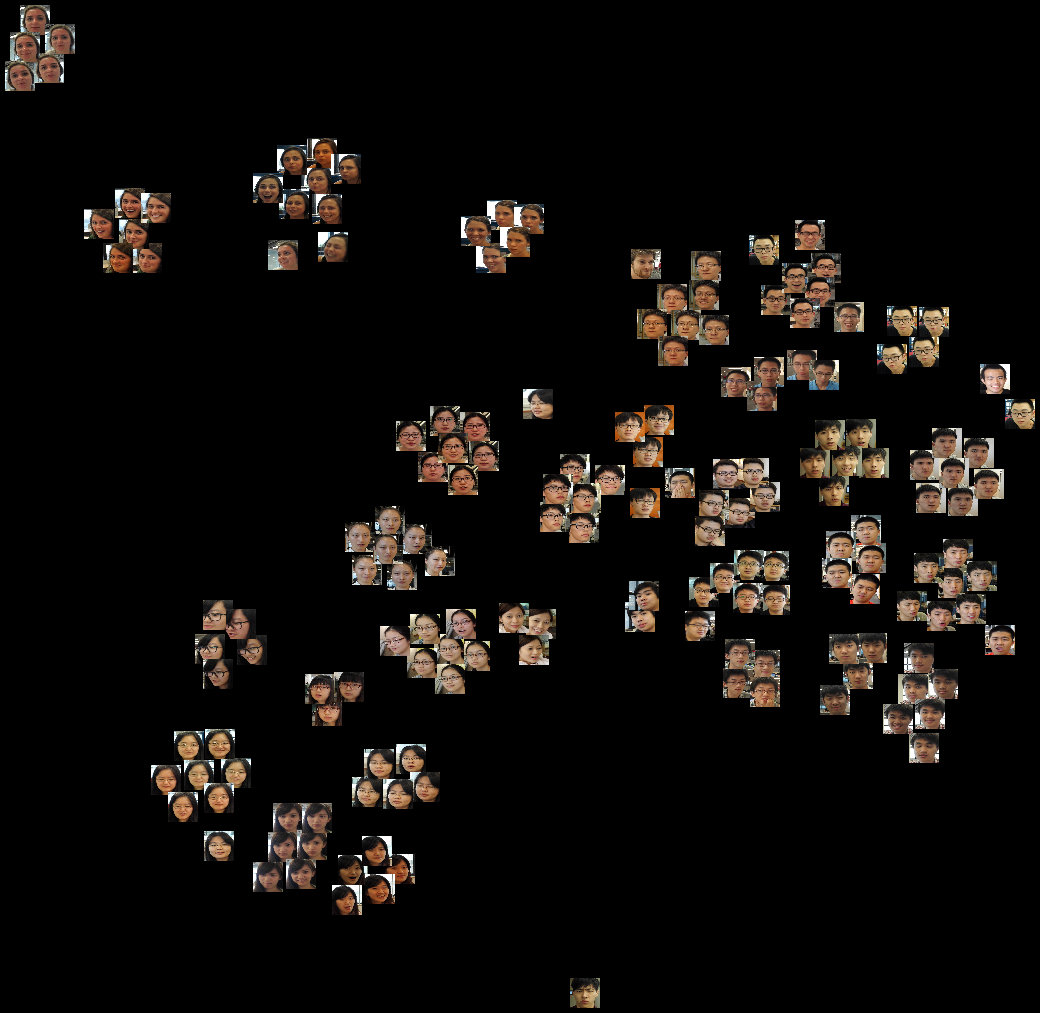
\includegraphics[height=0.5\textheight,keepaspectratio]{figure/ch4-tsnevggfc8.png}
        ~
        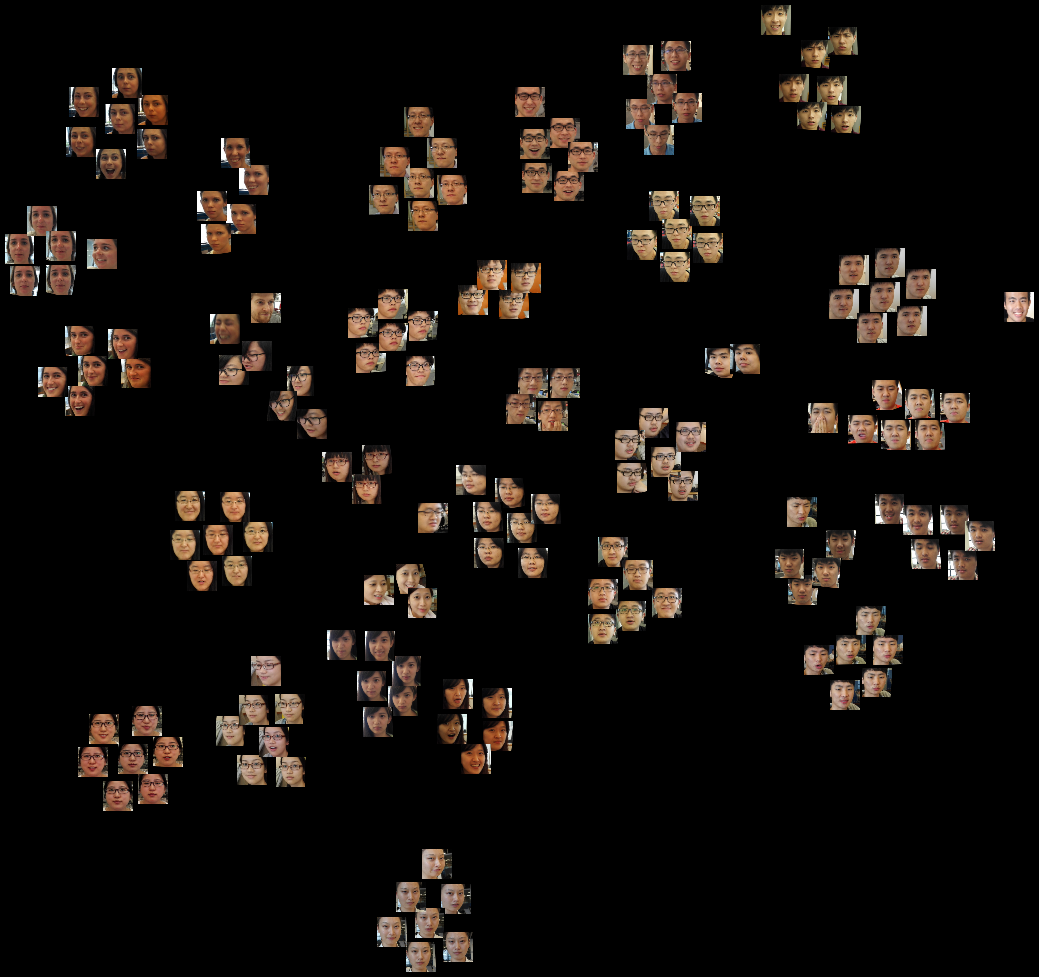
\includegraphics[height=0.5\textheight,keepaspectratio]{figure/ch4-tsnemfmeltwise_fc1.png}
    \end{figure}
}
\only<3>{

\begin{table}[!htbp]
\scriptsize
\centering
\caption{\tiny Time of single facial feature extraction and batch facial feature extraction (10 faces).}
% \label{tbl-forwardingtime}
\begin{tabular}{lrrr}
\toprule
 & Xiaomi Mi 3W & Galaxy Note 4 & Xiaomi Mi 5\\
 & {\tiny Snapdragon 800} & {\tiny Snapdragon 805} & {\tiny Snapdragon 820}\\
 & {\tiny 2GB RAM} & {\tiny 3GB RAM} & {\tiny 4GB RAM}\\
 \midrule
1 VGG CNN & N/A & N/A & $\sim 2780$ ms \\
10 VGG CNN & N/A & N/A & $\sim 26740$ ms \\
1 Lightened CNN & $\sim 508$ ms & $\sim 330$ ms & $\sim 303$ ms \\
10 Lightened CNN & $\sim 6602$ ms & $\sim 3071$ ms & $\sim 2031$ ms \\
 \bottomrule

\end{tabular}
\end{table}

}

\only<4>{
\vspace{0.5cm}
\begin{block}{\bf Detection and alignment}
  \easyfigure{figure/ch4-facedetalign.pdf}
\end{block}

\begin{block}{\bf Recognition model}
  {\centering \scriptsize \color{blue} SVM, probability threshold $T_p$ at prediction time}
\end{block}
}

\only<5>{
\vspace{0.5cm}
\begin{block}{\bf Face matching algorithm}

{\scriptsize \color{blue} Distance metric: $\mathtt{cosine}$ }

\begin{algorithm}[H]
% \caption{Face Matching}
% \label{alg:face}
\begin{algorithmic}[1] %show line numbers
\begin{scriptsize}
\STATE initialize \textit{P's} feature $f_0$, \textit{Bob's} feature $f_{i}, i \in 1, \ldots, N$, distance threshold $T_d$, hit ratio threshold $T_r$ % number of \textit{Bob's} features $N$
\STATE $m \gets 0$ $//$ number of hits
\FOR{$i=1$ to $N$}
	\STATE $d_{i} \gets dis(f_{0},f_{i})$ $//$ $dis(x,y)$ returns the distance between $x$ and $y$
	%\STATE $//$ $dis(x,y)$ returns the distance between $x$ and $y$
	\IF{$d_{i} \leq T_{d}$}
		\STATE $m \gets m + 1$
 	\ENDIF
\ENDFOR
\IF{$m / N \geq T_{r}$}
    \RETURN true $//$ \textit{P} is \textit{Bob}
\ELSE %$//$ $p \neq q$
    \RETURN false $//$ \textit{P} and \textit{Bob} are two persons
\ENDIF
\end{scriptsize}
\end{algorithmic}
\end{algorithm}


\end{block}

}

\end{frame}

\begin{frame}[t]
\setbeamercovered{transparent}
\setbeamercolor{alerted text}{fg=blue}
\frametitle{Gesture recognition}
\begin{columns}[T]
\begin{column}{0.4\textwidth}
  \begin{block}{\bf Training}
    \begin{itemize}
        \item<1-|alert@+> Dataset
        \item<2-|alert@+> Pre-trained model
        \item<3-|alert@+> Train detector
    \end{itemize}
  \end{block}

  \only<1->{\tiny\color{blue} VGG hand dataset:  5628 images with 13050 ``natural'' gesture instances, {\em \url{http://www.robots.ox.ac.uk:5000/~vgg/research/hands/index.html}}

  \vspace{0.5cm}Self prepared dataset: 4712 images with ``yes'' gestures and 3503 images with ``no'' gestures}

  \only<2->{\vspace{0.5cm} VGG16 ImageNet model}

  \only<3->{\vspace{0.5cm} Fine tune ``conv3\_1'' and up layers, approximate joint optimization}

\end{column}\hfill

\begin{column}{0.6\textwidth}
  \vspace{-0.5cm}
  \begin{block}{\centering\bf Composed dataset}
    \easyfigure[0.7]{figure/ch4-gesturedataset.png}
  \end{block}
\end{column}

\end{columns}
\end{frame}

\begin{frame}[t]
\frametitle{Gesture recognition}
\vspace{-0.5cm}
\begin{block}{\bf Prediction examples}
  \easyfigure[0.75]{figure/ch4-gestpredemp.png}
\end{block}

\end{frame}

\subsection{Integration}

\begin{frame}[t]
\frametitle{Decision flow}
\only<1>{
\begin{block}{\bf Decision path of protection action}
  \easyfigure[0.7]{figure/ch4-decisiontree.pdf}
\end{block}
}

\only<2>{
\begin{block}{\bf Example}
\begin{figure}[!htbp]
  \makebox[\textwidth]{
    \centering
    \raisebox{-0.5\height}{
      \begin{subfigure}[b]{0.55\textwidth}
        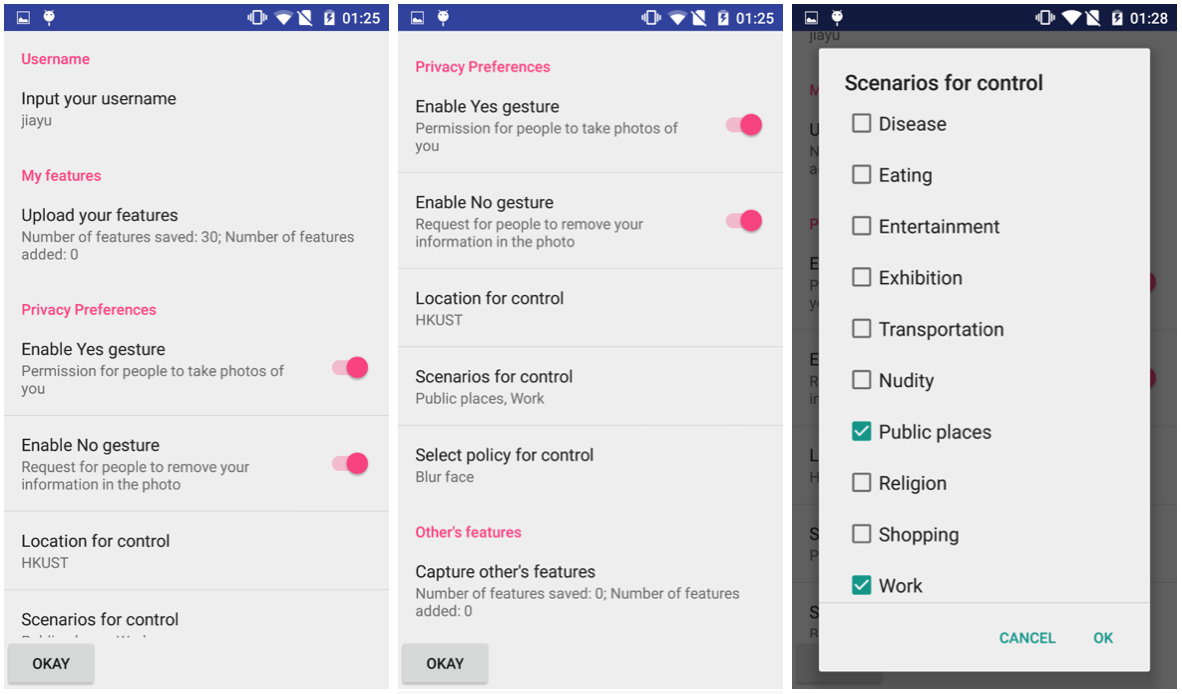
\includegraphics[width=\textwidth]{figure/ch4-reg.png}
        \caption{\scriptsize Registration and profile updating interface}
        \label{fig:ch4-reg}
      \end{subfigure}
    }
    \raisebox{-0.5\height}{
      \begin{subfigure}[b]{0.43\textwidth}
        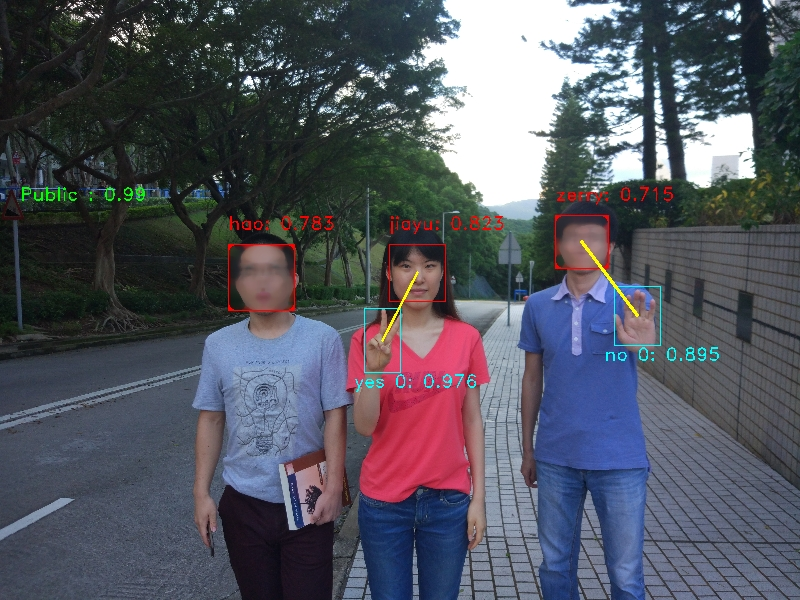
\includegraphics[width=\textwidth]{figure/ch4-allres.jpg}
        \caption{\scriptsize Privacy protection example}
        \label{fig:ch4-allres}
      \end{subfigure}
    }
  }
  \vspace{-0.25cm}
  \caption{\tiny Cardea user interface and privacy protection results. In (a), \textit{jiayu} registers as a Cardea user by extracting and uploading her face features. She specifies HKUST, two scene groups for privacy protection. She also enables ``yes'' and ``no'' gestures. In (b), a picture is taken in HKUST. 3 registered users, one ``yes'' and one ``no'' gesture are recognized. The scene is correctly predicted as ``Public''. \textit{jiayu}'s face is not blurred due to her ``yes'' gesture. Prediction probabilities are also shown in (b).}
  % \label{fig:ch4-uires}
\end{figure}
\end{block}
}

\end{frame}

\begin{frame}[t]
\frametitle{System overview}

\begin{columns}[T]
\begin{column}{0.44\textwidth}
  \begin{block}{\bf On mobile}
    \begin{itemize}
      \item face detection, alignment
      \item face feature extraction
      \item scene classification
    \end{itemize}
    {\scriptsize  OpenCV, Dlib, Caffe-android-lib}
  \end{block}
\end{column}\hfill
\begin{column}{0.5\textwidth}
  \begin{block}{\bf On cloud}
    \begin{itemize}
      \item face recognition
      \item face recognition model updating
      \item gesture recognition
    \end{itemize}
    {\scriptsize Py-faster-rcnn, LIBSVM, multiprocessing/multithreading}
  \end{block}
\end{column}
\end{columns}

\vspace{1cm}
{\scriptsize  Demo video link: \em http://bit.ly/2egw2H6}


\end{frame}



\section{System Evaluation}
\frame{\frametitle{Agenda} \tableofcontents[currentsection]}

\subsection{Vision Performances}
\begin{frame}[t]
\frametitle{Scene classification}
\only<1>{
\vspace{-0.25cm}
\begin{block}{\bf Scene group modification}
\begin{table}[tb]
\tiny
\centering
% \caption{Nine general scene groups}
% \label{tbl-scenecateupdate}
\begin{tabular}{llll}
\toprule
\textbf{Group name}  & \textbf{Abbreviatin}    & \textbf{Scenes \#}     & \textbf{Examples}   \\ \midrule
Shopping        &Sh & $20$            & clothing store, market, supermarket\\ \midrule
Travelling      &Tr & $9$             & airport, bus station, subway platform\\ \midrule
Park \& street  &Pa & $12$            & downtown, park, street, alley\\ \midrule
Eating \&       &Ea & $18$            & bar, bistro, cafeteria, coffee shop,\\
drinking        & &                 & fastfood restaurant, food court\\ \midrule
Working \&      &Wo & $9$             & classroom, conference center, library,\\
study           & &                 & office, reading room\\ \midrule
Scantily clad   &Sc & $12$            & beach, swimming pool, water park\\ \midrule
Medical care    &Me & $2$             & hospital room, nursing home\\ \midrule
Religion        &Re & $11$            & cathedral, chapel, church, temple\\ \midrule
Entertainment   &En & $5$             & amusement park, ballroom, discotheque\\ \midrule
\textit{All}    & & $\mathit{98}$   &   \\ \bottomrule
\end{tabular}
\end{table}
\vspace{-0.25cm}
{\scriptsize \color{blue} Add more scenes, remove ``Exhibition'' group. Train the new model, 55\% and 83\% validation accuracy. Evaluation results are based on new model.}
\end{block}
}

\only<2>{
  \vspace{-0.25cm}
  \begin{block}{\bf Group recall}

\begin{figure}[!htbp]
  \makebox[\textwidth]{
    \centering
    \raisebox{-0.5\height}{
      \begin{subfigure}[b]{0.48\textwidth}
        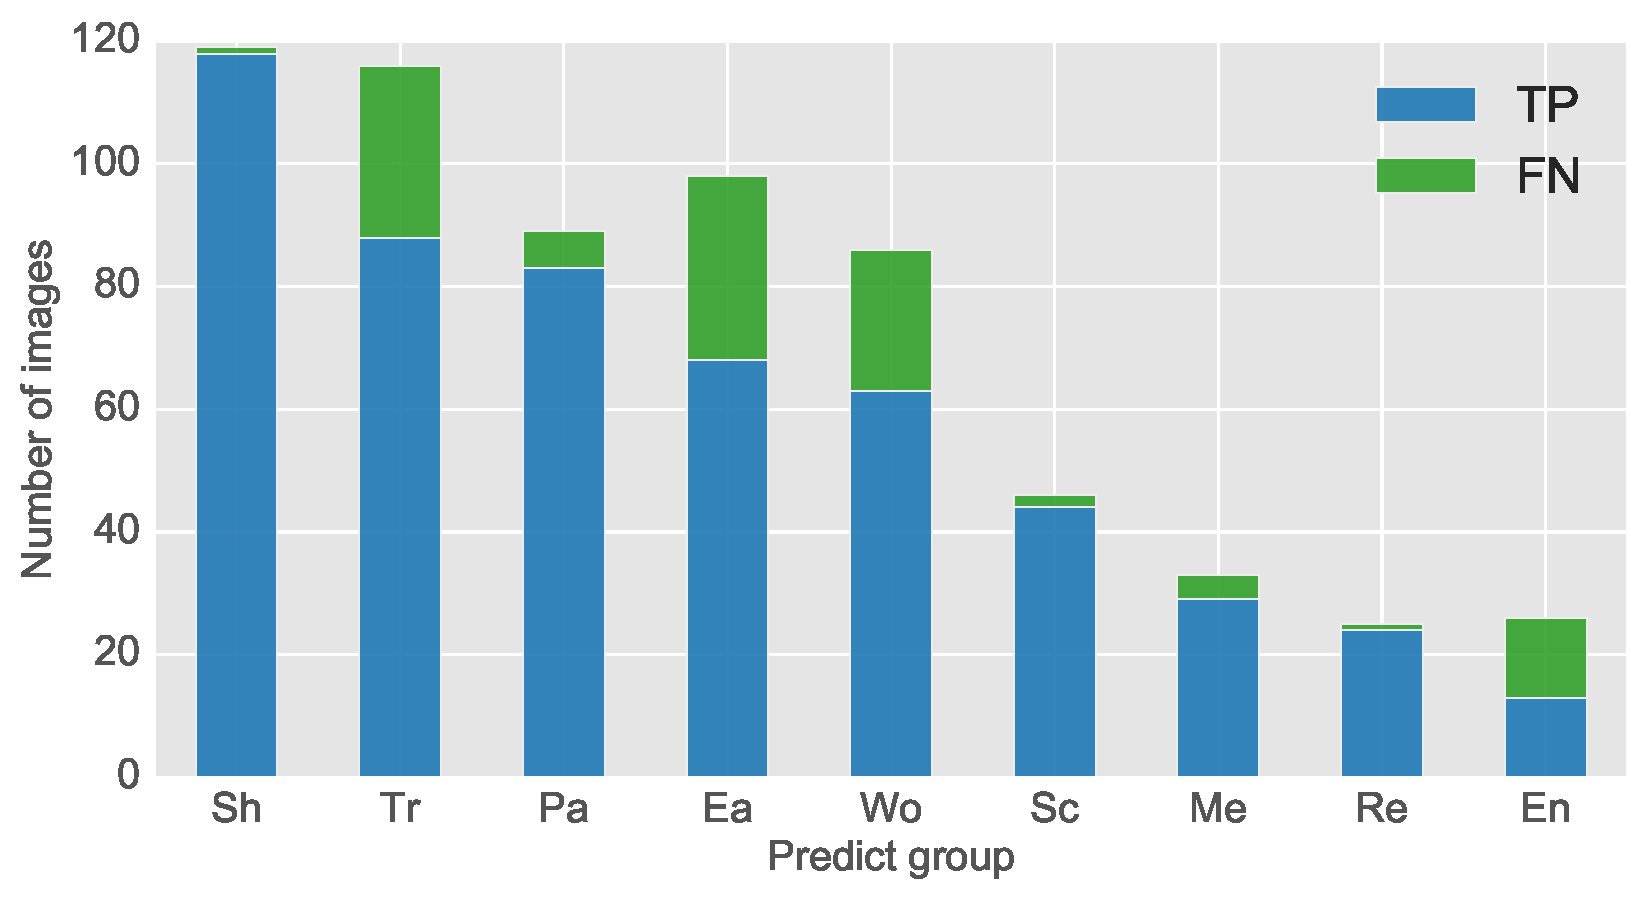
\includegraphics[width=\textwidth]{figure/ch4-scenerecall.pdf}
        \caption{\tiny Recall}
        % \label{fig:ch4-scenerecall}
      \end{subfigure}
    }
    \raisebox{-0.5\height}{
      \begin{subfigure}[b]{0.48\textwidth}
        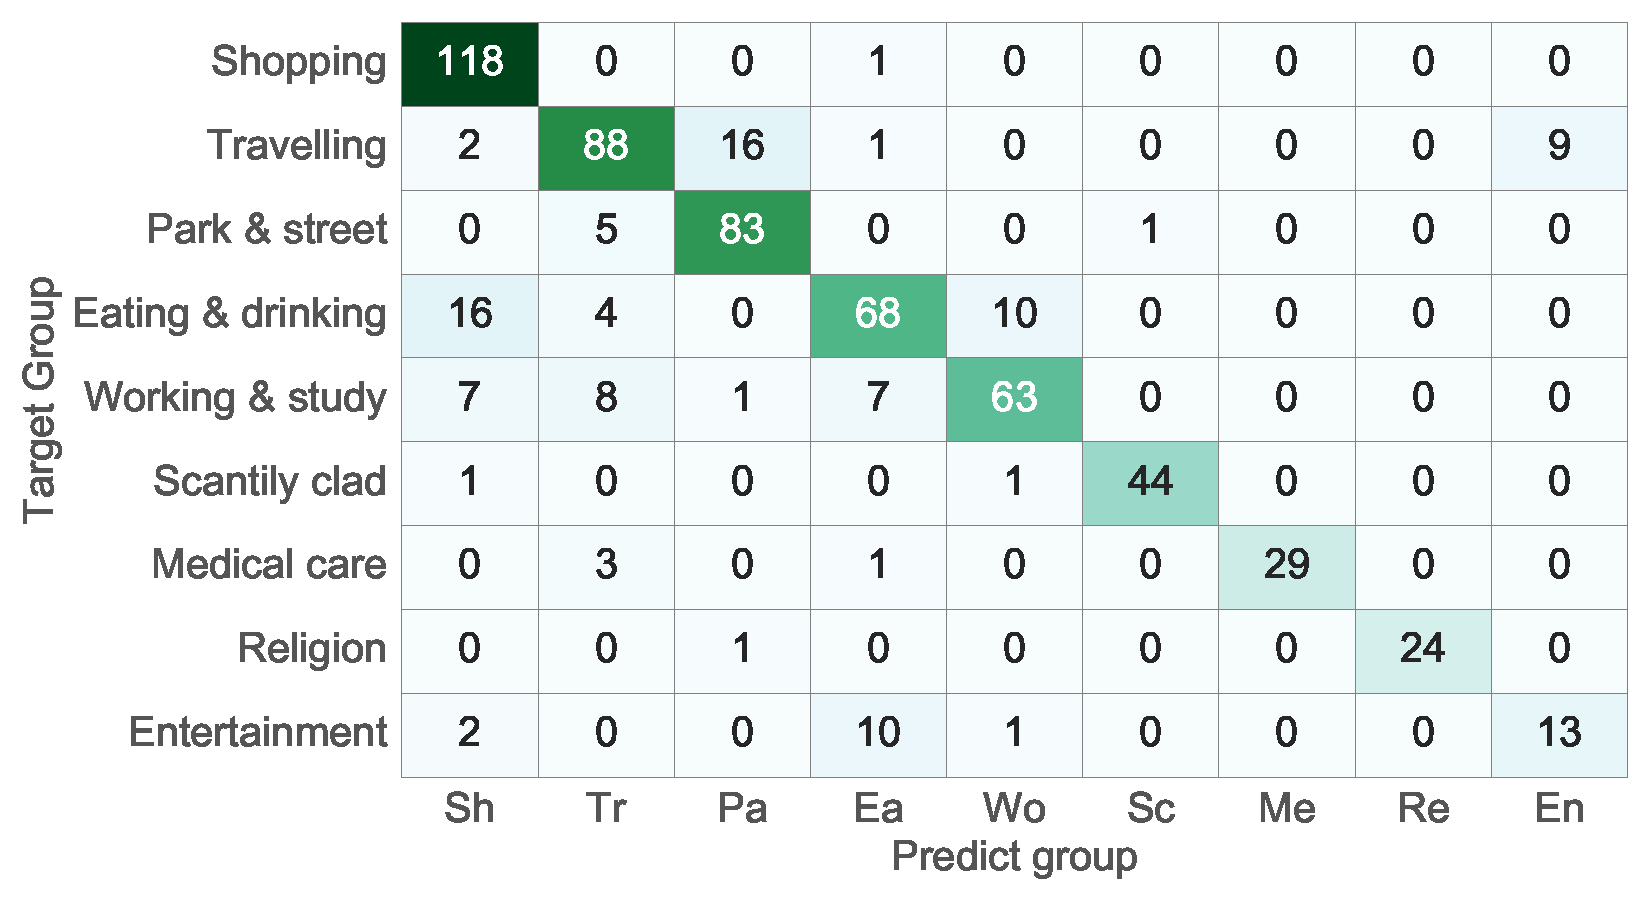
\includegraphics[width=\textwidth]{figure/ch4-sceneconfusion.pdf}
        \caption{\tiny Confusion matrix}
        % \label{fig:ch4-sceneconfusion}
      \end{subfigure}
    }
  }

\caption{\scriptsize Scene classification evaluation results.}
% \label{fig:ch4-sceneeval}
\end{figure}

{\scriptsize \color{blue} 8 volunteers take 759 images in ``in the wild'', with 638 images are selected, covering 9 scene groups shown earlier.}
  \end{block}
}
\end{frame}

\begin{frame}[t]
\frametitle{Face recognition and matching}
\vspace{-0.25cm}
\only<1>{
\begin{block}{\bf Recognition accuracy with $T_p$}

\begin{figure}[!htbp]
  \makebox[\textwidth]{
    \centering
    \raisebox{-0.5\height}{
      \begin{subfigure}[b]{0.48\textwidth}
        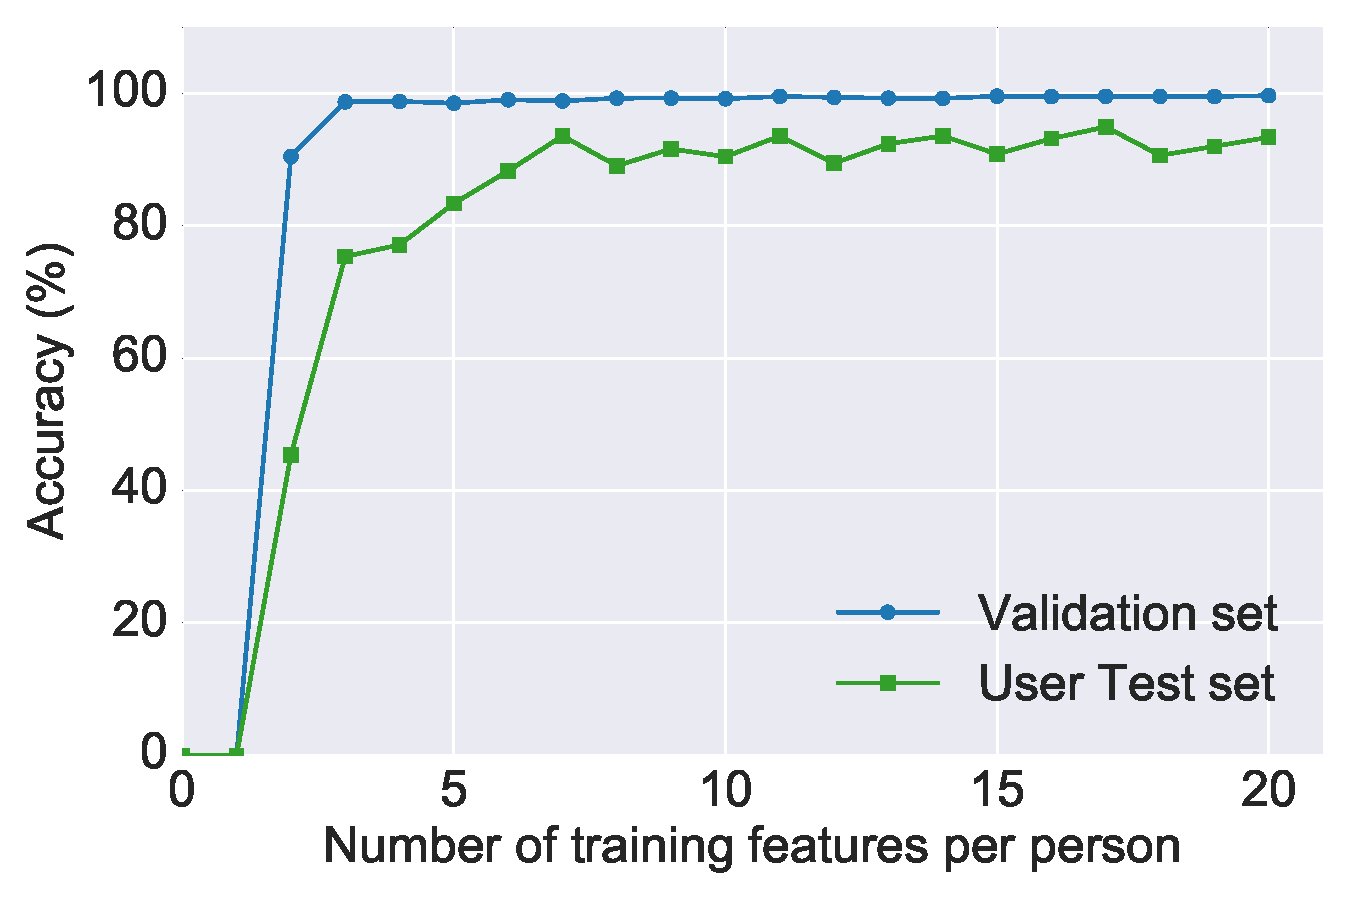
\includegraphics[width=\textwidth]{figure/ch4-accuracy-num.pdf}
        \caption{\tiny Training accuracy}
        % \label{fig:ch4-accnum}
      \end{subfigure}
    }
    \raisebox{-0.5\height}{
      \begin{subfigure}[b]{0.48\textwidth}
        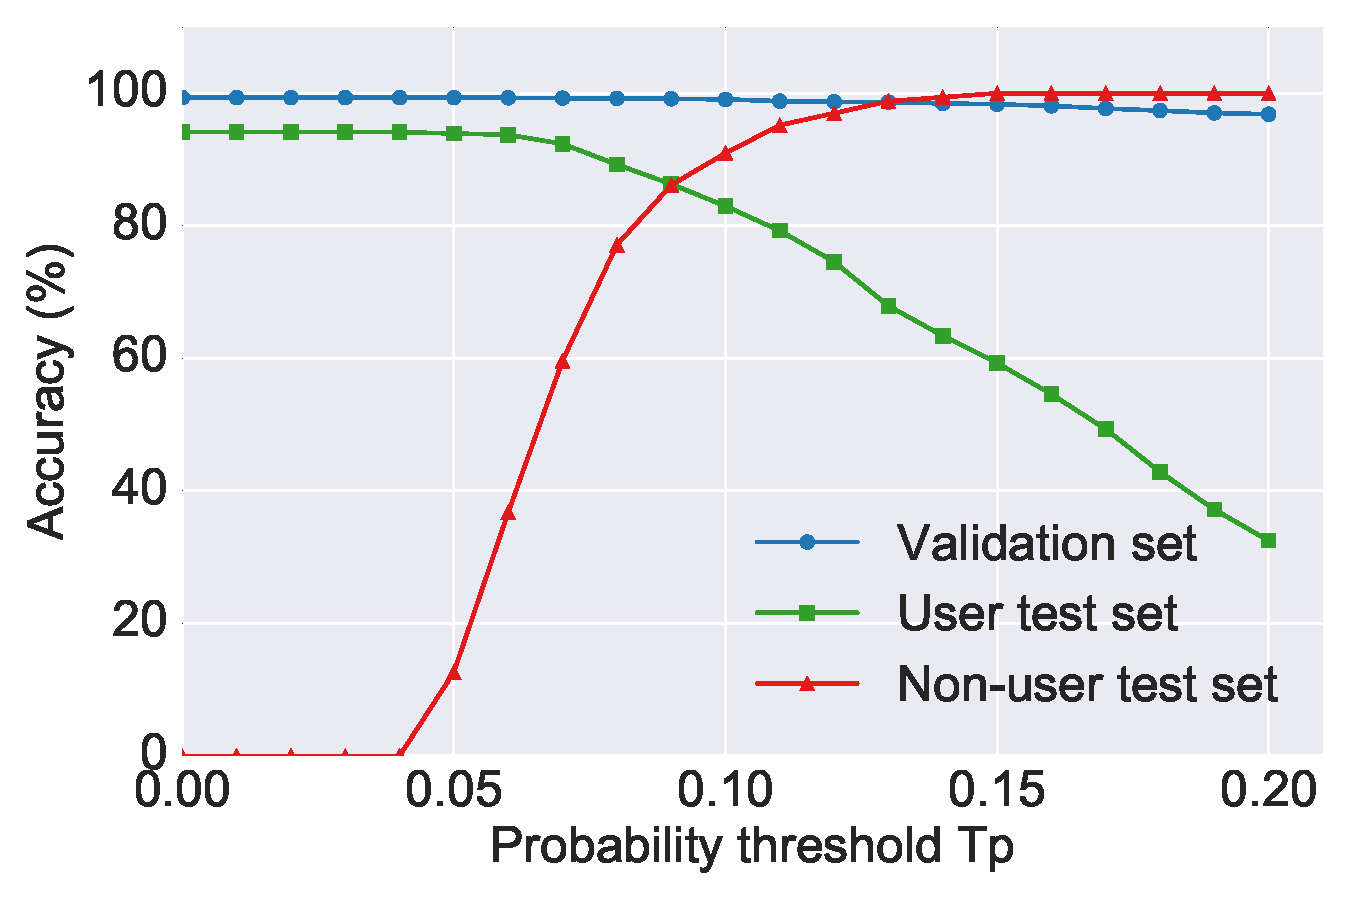
\includegraphics[width=\textwidth]{figure/ch4-accuracy-threshold.pdf}
        \caption{\tiny Testing accuracy with threshold $T_p$}
        % \label{fig:ch4-accthreshold}
      \end{subfigure}
    }
  }
% \caption{Face recognition accuracy.}
% \label{fig:ch4-facereceval}
\end{figure}

\vspace{-0.5cm}{\scriptsize \color{blue} Select 50 subjects from LFW dataset, 5042 features for train and validation, 511 features as {\bf\color{purple} user test set}, 166 features from 100 other subjects as {\bf\color{purple} non-user test set}. (CASIA WebFace Database (Lightene CNN) does not overlap with LFW dataset). }

\end{block}
}


\only<2>{
\begin{block}{\bf Matching accuracy with $T_d$ \& $T_r$}

\begin{figure}[!htbp]
  \makebox[\textwidth]{
    \centering
    \raisebox{-0.5\height}{
      \begin{subfigure}[b]{0.48\textwidth}
        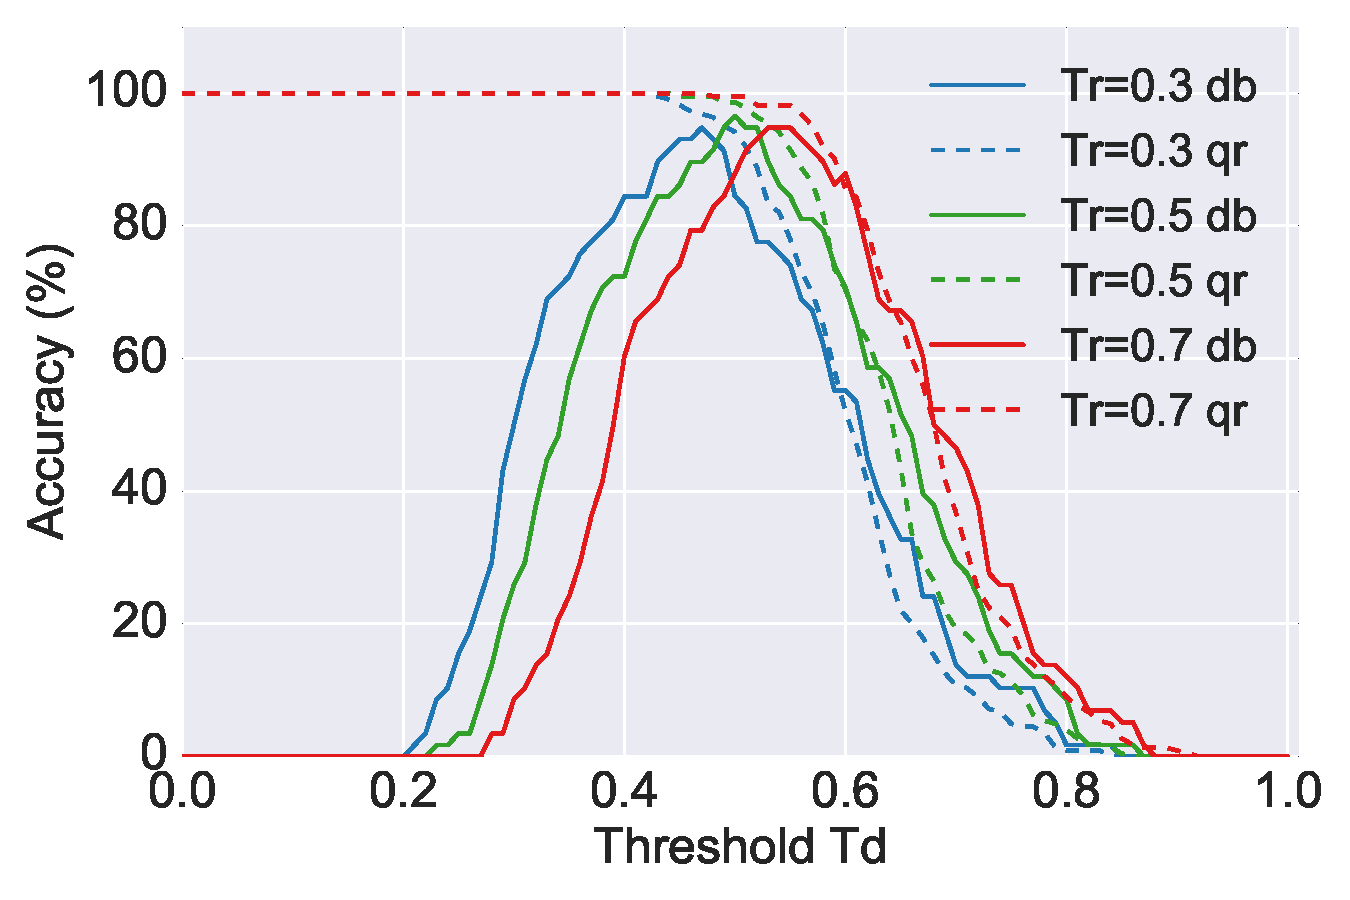
\includegraphics[width=\textwidth]{figure/ch4-accuracy-cosine.pdf}
        \caption{\tiny Cosine distance}
        % \label{fig:ch4-acccosine}
      \end{subfigure}
    }
    \raisebox{-0.5\height}{
      \begin{subfigure}[b]{0.48\textwidth}
        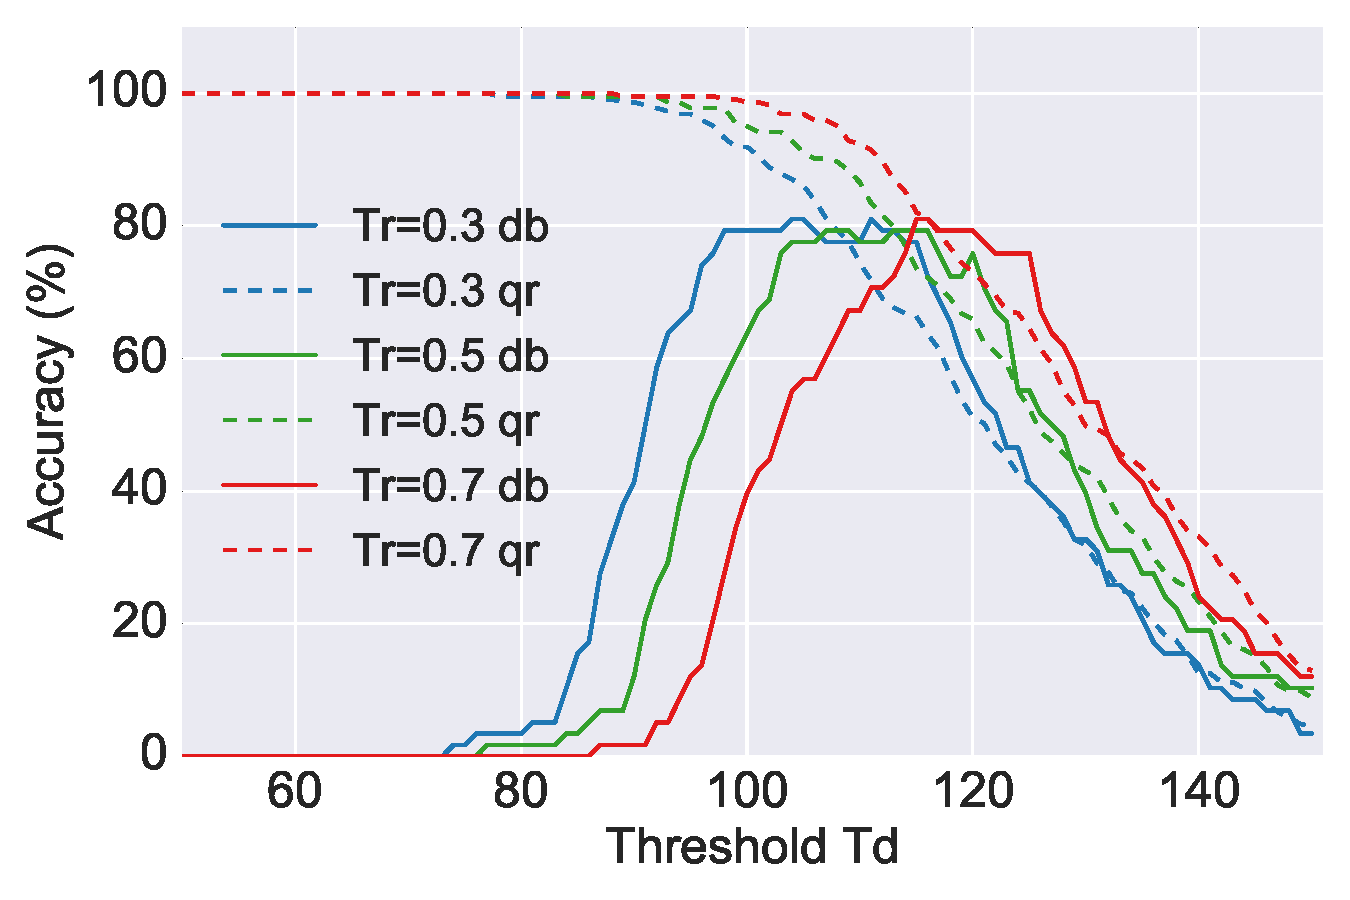
\includegraphics[width=\textwidth]{figure/ch4-accuracy-l2.pdf}
        \caption{\tiny Euclidean distance}
        % \label{fig:ch4-accl2}
      \end{subfigure}
    }
  }
% \caption{Face matching accuracy with different distance threshold $T_d$ and ratio threshold $T_r$.}
% \label{fig:ch4-facematcheval}
\end{figure}

\vspace{-0.5cm}{\scriptsize \color{blue} Select 23 subjects from {\bf\color{purple} user test set} who has more than 10 features, use these 230 features as {\bf\color{purple} database group} (solid line), the other 281 features as {\bf\color{purple} query group} (dashed line).}

\end{block}
}

\end{frame}

\begin{frame}[t]
\frametitle{Gesture recognition}

\vspace{-0.25cm}
\begin{block}{\bf Recognition performance to scene and gesture region size}
\begin{figure}[!htbp]
  \makebox[\textwidth]{
    \centering
    \raisebox{-0.5\height}{
      \begin{subfigure}[b]{0.32\textwidth}
        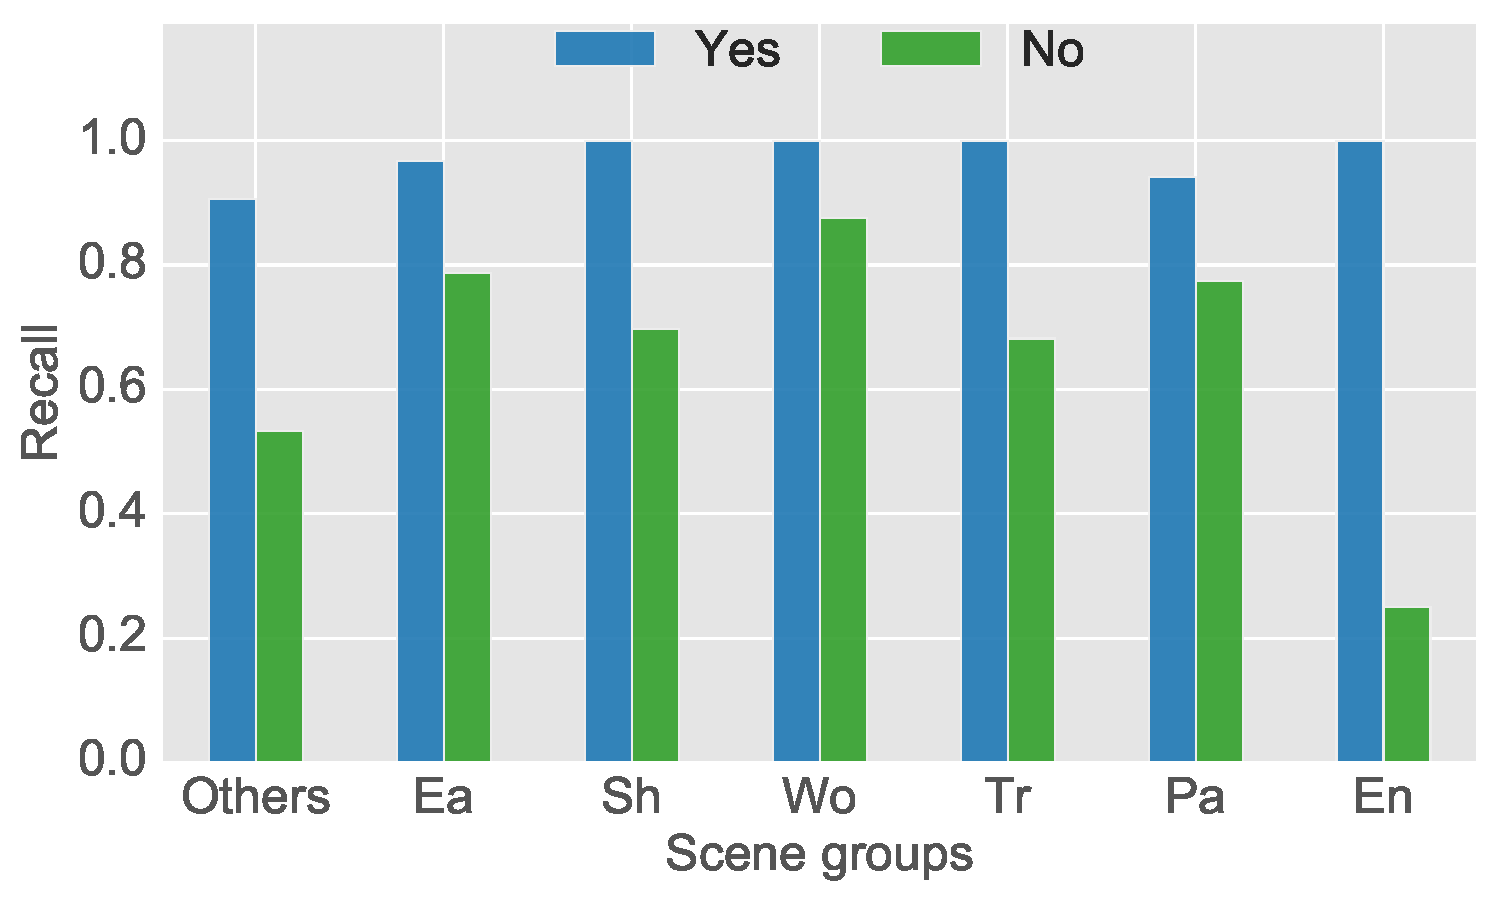
\includegraphics[width=\textwidth]{figure/ch4-hand-recall.pdf}
        \caption{\tiny Recall for different scenes}
        % \label{fig:ch4-gestrecallscn}
      \end{subfigure}
    }
    \raisebox{-0.5\height}{
      \begin{subfigure}[b]{0.32\textwidth}
        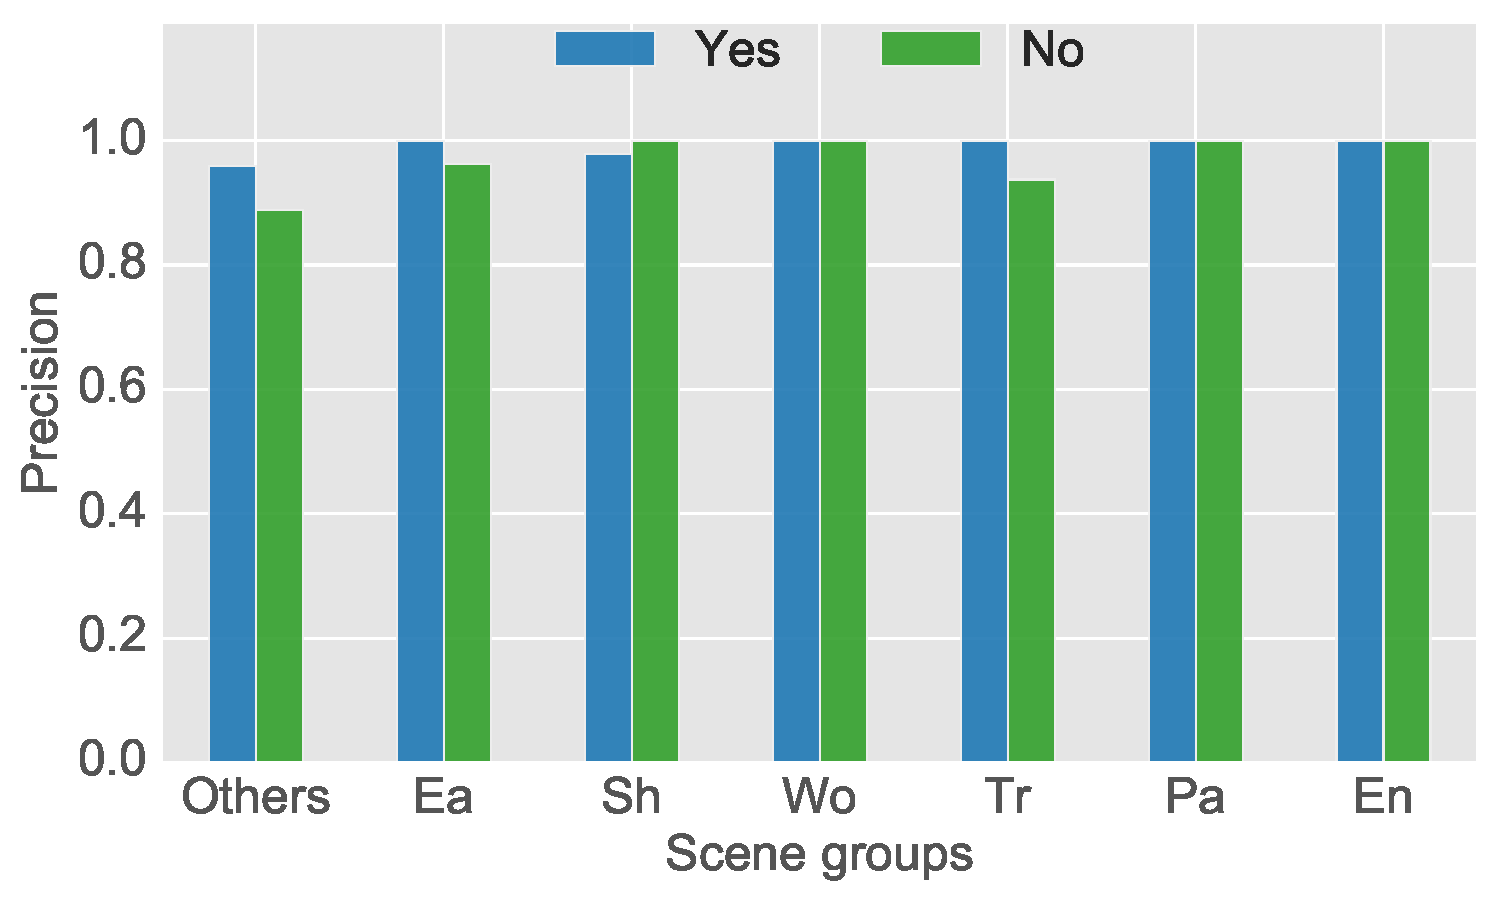
\includegraphics[width=\textwidth]{figure/ch4-hand-precision.pdf}
        \caption{\tiny Precision for different scenes}
        % \label{fig:ch4-gestprecisionscn}
      \end{subfigure}
    }
    \raisebox{-0.5\height}{
      \begin{subfigure}[b]{0.32\textwidth}
        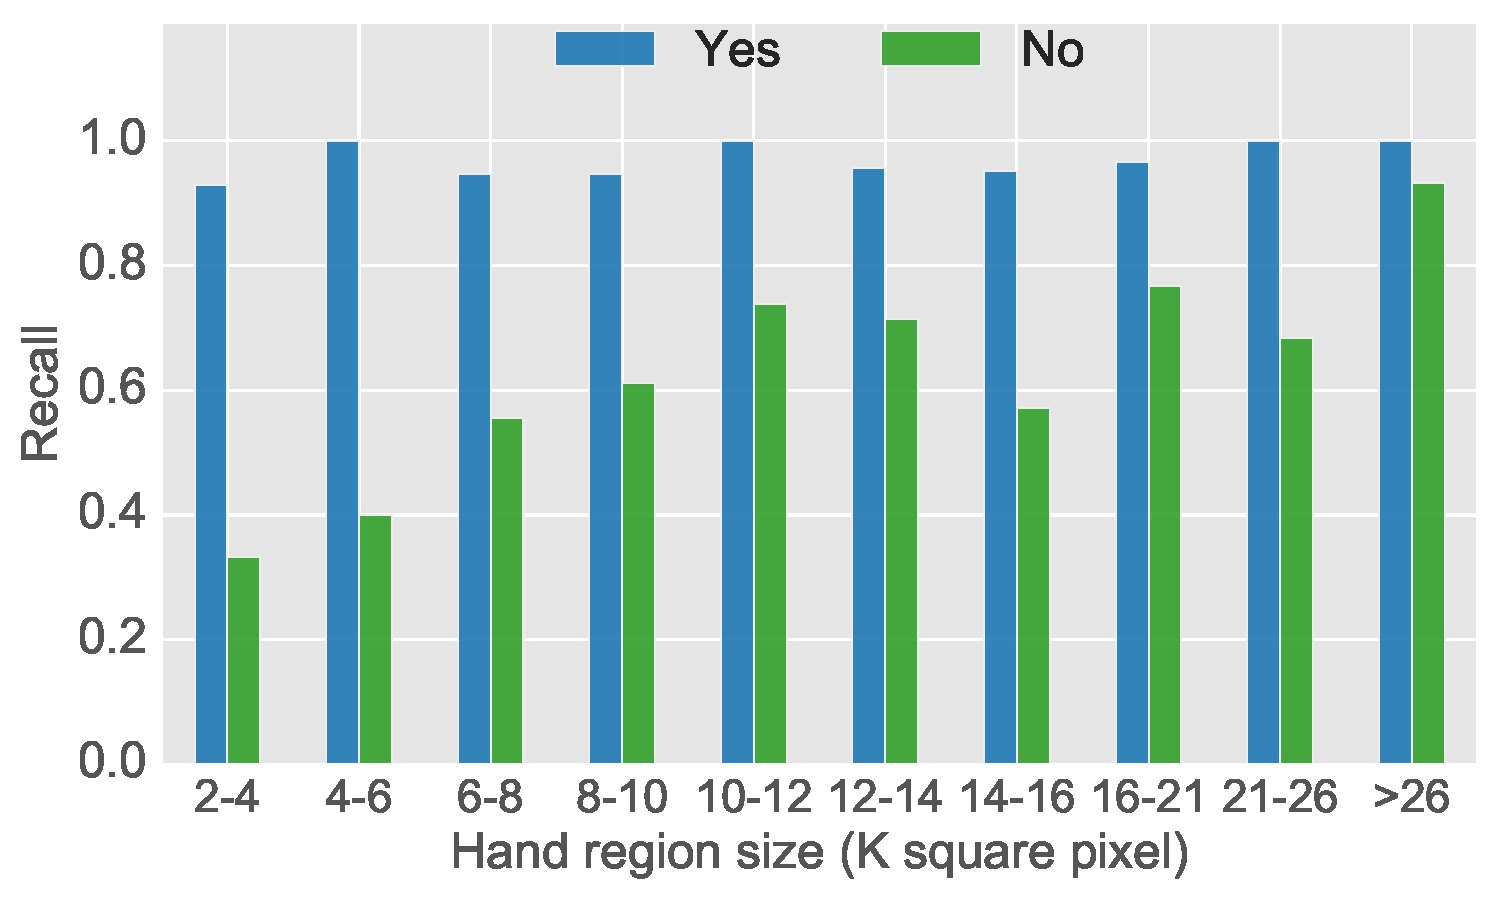
\includegraphics[width=\textwidth]{figure/ch4-hand-recall-size.pdf}
        \caption{\tiny Recall for different hand region sizes}
        % \label{fig:ch4-gestrecallsize}
      \end{subfigure}
    }
  }
% \caption{Hand gesture recognition results.}
% \label{fig:ch4-gesteval}
\end{figure}
\vspace{-0.5cm}{\scriptsize \color{blue} High precision, recall for ``no'' gesture needs to be improved. More training data with smaller size.}
\end{block}

\end{frame}

\begin{frame}[t]
\frametitle{Overall protection accuracy}

\begin{table}[tb]
\centering
\caption{Cardea's overall privacy protection performance.}
% \label{tbl-overallperform}
\begin{tabular}{lr|lr}
\toprule
\textbf{Overall accuracy}   & $\mathbf{86.4\%}$ & Protection accuracy   & $80.4\%$  \\
                            &                   &  No protection accuracy& $91.0\%$ \\ \midrule
Face recognition accuracy   & $98.5\%$  & ``Yes'' gesture recall        & $97.9\%$  \\
scene classification recall & $77.7\%$  & ``No'' gesture recall     & $77.3\%$  \\ \bottomrule

\end{tabular}
\end{table}


{\scriptsize \color{blue} 5 volunteers to register as Cardea users, set their privacy profiles. 224 images for evaluation.}

%% 122 / (122 + 12)
%% 82 / (82 + 20)

\end{frame}

\subsection{Runtime \& Energy Consumption}
\begin{frame}[t]
\frametitle{Runtime}

\vspace{-0.25cm}
\begin{figure}[tb]
\centering
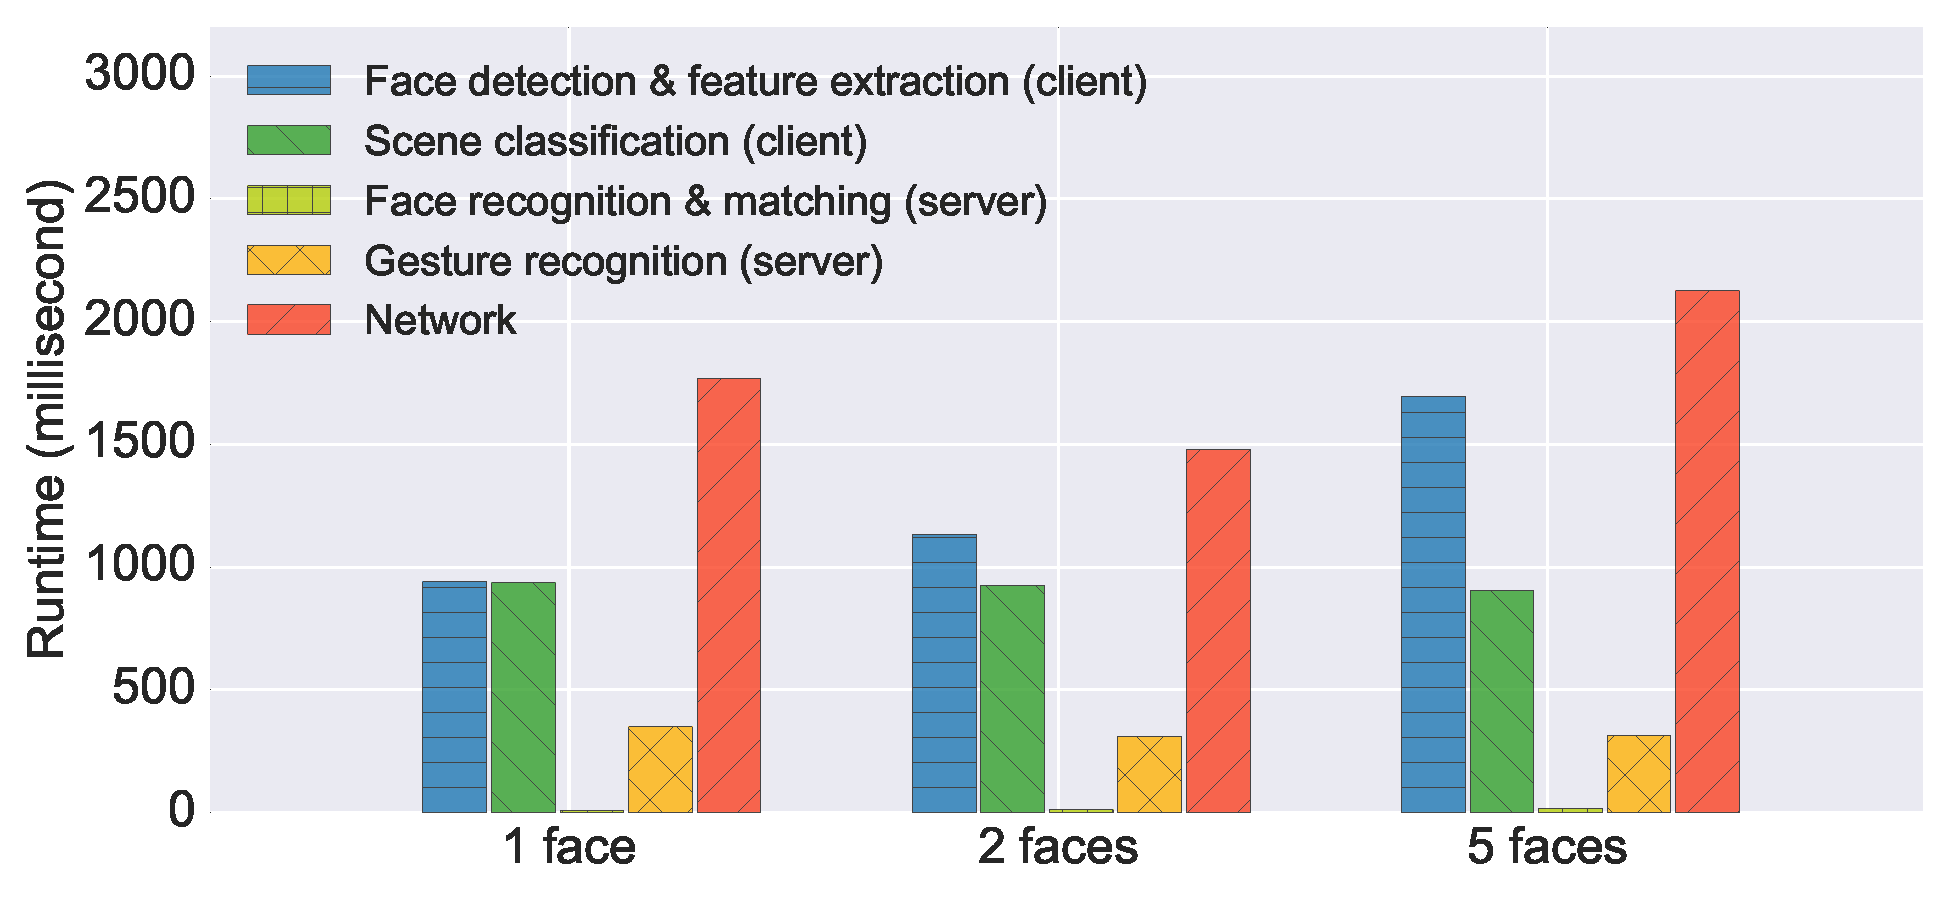
\includegraphics[width=0.8\textwidth]{figure/ch4-runtime.pdf}
\caption{Task level runtime of Cardea.}
% \label{fig:ch4-runtime}
\end{figure}

\vspace{-0.5cm}{\scriptsize \color{blue} client: Samsung Galaxy Note 4, 4$\times$2.7 GHz Krait 450 CPU, Qualcomm Snapdragon 805 Chipset, 3GB RAM, and 16 MP, f/2.2 Camera.}\\

{\scriptsize \color{blue} server: Intel i7--5820K CPU, 16GB RAM, GeForce 980Ti Graphic Card (6GB RAM).}\\

{\scriptsize \color{blue} network: eduroam.}

\end{frame}

\begin{frame}[t]
\frametitle{Energy consumption}

\begin{table}[tb]
\centering
\caption{Energy consumption of Cardea with different number of faces.}
% \label{tbl-energy}
\begin{tabular}{lrrr}
\toprule
            & Face recognition      & Whole process (uAh)   & \# of images \\ \midrule
1 face      & $217.2$ (std $3.4$)   & $1134.5$ (std $45.9$) & $\sim 2800$       \\
2 faces     & $344.1$ (std $13.1$)  & $1276.7$ (std $113.8$)    & $\sim 2500$       \\
5 faces     & $692.6$ (std $36.5$)  & $1641.1$ (std $66.0$) & $\sim 2000$       \\ \bottomrule
\end{tabular}
\end{table}

\end{frame}

\section{Conclusion}
\frame{\frametitle{Agenda} \tableofcontents[currentsection]}

\begin{frame}
\frametitle{Summary}
\begin{itemize}
\item Design
\begin{itemize}
    \item context awareness
    \item interactive control
\end{itemize}

\item Implementation
\begin{itemize}
    \item deep neural networks
    \item deploy on android
\end{itemize}

\item Feasibility
\begin{itemize}
    \item micro benchmarks
    \item overall performance
    \item run time \& energy consumption
\end{itemize}


\end{itemize}

\end{frame}

% \begin{frame}
% \frametitle{Future work}

% \end{frame}

\begin{frame}
\begin{center}
\huge
Thanks for your attendance ! \\
Q\&A ?
\end{center}

\end{frame}


% \begin{frame}[t]
% \frametitle{Slide template}
% \begin{columns}[T]
% \begin{column}{0.5\textwidth}
  % \begin{block}{\bf Block up}

  % \end{block}

  % \begin{block}{\bf Block down}

  % \end{block}
% \end{column}\hfill

% \begin{column}{0.5\textwidth}
% \end{column}
% \end{columns}
% \end{frame}


\end{document}
